\documentclass[12pt,a4paper,oneside,openright]{report} % twosided
\usepackage{../../../../LaTeX/general}

\title{\vspace{-8ex}Derivation of the CELMA equations\vspace{-1ex}}
\author{Michael L{\o}iten}
\date{\vspace{-2ex}\today}

\pagestyle{fancy}
\fancyhf{}
\lhead{}
\chead{}
\rhead{\rightmark}
\cfoot{\thepage}
\renewcommand{\sectionmark}[1]{\markright{#1}{}}
% \usepackage{draftwatermark}
% \SetWatermarkLightness{0.7}
% \SetWatermarkScale{4}
%+++++++++++++++++++++++++++++++++++++++++++++++++++++++++++++++++++++++++++++++

%===================================================
\everymath{\displaystyle}
\usepackage{titlesec}
%\titleformat*{\section}{\bfseries}%\vspace{-0.2cm}}


% Section without numbering
%\renewcommand\thesection{\hspace{-0.5cm}}
%===================================================

% Nice tables
\renewcommand{\arraystretch}{1.5}


% Shorcuts for this document
\def\vt{\ve{\vartheta}}
% References

\begin{document}
\maketitle
%
\chapter{The kinetic equation}
We will here derive the fluid equations used in the rest of this thesis from the Fokker-Planck%
\footnote{
    This equation can again be derived from the Klimontovich equation (see for example \cite{Klimontovich1983book}).
}
%
 equation by following the approach of \cite{Helander2002book}.
In addition we will include an inelastic source.
This source will either add or subtract particles to the distribution function depending on its sign.

We are looking at a distribution function $f_\a(\ve{r},\ve{v},t)$ of species $\a$, at point $\ve{z}(t)=(\ve{r}(t),\ve{v}(t))$ in the phase-space at time $t$.
The particles obey the conservation equation
%
\begin{align*}
    \partial_t f_\a + \partial_{\ve{z}} \L(\L[\d_t \ve{z}\R]f_\a\R) =& S'_\a,
\end{align*}
%
where $S'_\alpha$ is a source in the distribution function for species $\a$.
We will here use a source which fulfills the following:
%
\begin{align*}
    &\inde{S'_{\a}}{^3v} = S_{n,\a}&
    &\text{Particles are created.}&
    \\
    &\inde{m_\a \ve{v} S'_\a}{^3v} = 0&
    &\text{They are created with zero bulk velocity.}&
    \\
    &\inde{\frac{m_\a \ve{v}^2}{2} S'_\a}{^3v} = S_{E,\a}&
    &\text{They have a finite energy when created.}&
\end{align*}
%
Using that
%
\begin{align*}
    \d_t \ve{r}     =& \ve{v}\\
    \d_t \ve{v}     =& \frac{q_\a}{m_\a}\L(\ve{E}'+\ve{v}\times\ve{B}'\R)\\
    \partial_{\ve{v}} \L(\ve{E}'+\ve{v}\times\ve{B}'\R) =& 0,
\end{align*}
%
where $\ve{E}'$ and $\ve{B}'$ are the total (microscopic) fields, we get
%
\begin{align*}
      \partial_t f_\a
    + \ve{v}\cdot\nabla f_\a
    + \frac{q_\a}{m_\a}
      \L(\ve{E}'+\ve{v}\times\ve{B}'\R)\cdot\partial_{\ve{v}}f_\a
    =& S_\a.
\end{align*}

\section{Fokker-Planck equation}
We now introduce $\ve{E}$ and $\ve{B}$, which are the fields averaged over several Debye lengths.
To incorporate the microscopic fluctuations of the fields, we introduce the collision operator
%
\begin{align*}
    C_\a = \sum_\g C_{\a\g}(f_\a,f_\g)
\end{align*}
%
In the scope of this thesis, we will consider only elastic collisions between fully ionized, cold ions, electrons and cold neutrals (which only act as a static background).
In other words, we will let $\gamma \in \{e, i, n\}$ (denoting electrons, ions and neutrals), so that
%
\begin{align*}
    C_\a = C_{\a\b}(f_\a,f_\b) + C_{\a n}(f_\a,f_n)
\end{align*}
%
where $\a,\b \in \{e, i\}$ and $\a\neq \b$. Furthermore, the collision operator has the following properties:
%
\begin{align*}
    &\inde{C_{\a\g}}{^3v} = 0&
    &\text{Particle conservation}&
    \\
    &\inde{m_\a \ve{v} C_{\a\g}}{^3v} = -\inde{m_\a \ve{v} C_{\g\a}}{^3v}&
    &\text{Momentum conservation}&
    \\
    &\inde{\frac{m_\a \ve{v}^2}{2} C_{\a\g}}{^3v} =
    -\inde{\frac{m_\a \ve{v}^2}{2} C_{\g\a}}{^3v}&
    &\text{Energy conservation}&
\end{align*}
%
The resulting Fokker-Planck equation reads
%
\begin{empheq}[box=\tcbhighmath]{align}
      \partial_t f_\a
    + \ve{v}\cdot\nabla f_\a
    + \frac{q_\a}{m_\a}\L(\ve{E}+\ve{v}\times\ve{B}\R)\cdot\partial_{\ve{v}}f_\a
    = S_\a + C_\a.
    \label{eq:fp}
\end{empheq}

\section{Moments of Fokker-Planck}
To follow the distribution functions in a 6-dimensional phase-space as a function of time is quite a daunting task.
Instead, we will follow some averages of the distribution function.
This comes at the price of losing kinetic information in the system, like for example Landau damping.
We will use \cref{app:distAvg} to denote a weighted velocity average (a moment) of the Fokker-Planck equation, and note that $\expt{1}_{f_a}=n_a$ is the density of species $\a$.
From this, we define
%
\begin{align*}
    &\expt{\ve{v}_\a}_{f_a} \defined \; \ve{u}_a&  &\text{Macroscopic fluid velocity for }\a,&\\
    &\expt{m_\a n_\a \ve{v}_\a\ve{v}_\a}_{f_a} \defined\; \te{\Pi}_\a&  &\text{Momentum flux for }\a.&
\end{align*}
%
We call the difference between the velocity of a single particle and the macroscopic fluid velocity $\ve{w}$, so that
%
\begin{align*}
    \ve{w}_\a = \ve{v} - \ve{u}_\a.
\end{align*}
%
From this, we define the scalar pressure $p_\a$, the pressure tensor $\te{P}_\a$ and the stress tensor $\te{\pi}_\a$ as
%
\begin{align*}
    \frac{n_\a m_\a\expt{w_\a^2}_{f_a}}{3} \defined& \; p_\a = n_\a T_\a\\
    n_\a m_\a\expt{\ve{w}_{\a}\ve{w}_{\a}}_{f_a} \defined& \; \te{P}_\a\\
    \te{\pi}_\a \defined& \; \te{P}_\a - \te{I}p_\a\\
\end{align*}
%
where $\te{I}$ is the identity tensor.
Finally we define
%
\begin{align*}
    \inde{m_\a\ve{v} C_{\a\g}(f)}{^3v} \defined& \ve{R}_{\g\to\a},
\end{align*}
%
where $\ve{R}_{\g\to\a}$ is the friction force on $\a$ given by $\g$.

\subsection{Zeroth moment}
We will now work through the zeroth moment term by term by applying $\expt{n_\a \;\cdot\;}_{f_a}=n_\a\expt{\;\cdot\;}_{f_a}$ on \cref{eq:fp}.
We have that
%
\begin{align*}
    \expt{\partial_t n_\a}_{f_a}
    &=
    \partial_t n_\a \expt{1}_{f_a}
    \\
%
%
    &=
    \partial_t n_\a,
\end{align*}
%
that
%
\begin{align*}
    \expt{n_\a\ve{v}\cdot\nabla}_{f_a}
    &=
    \expt{n_\a\div\ve{v}}_{f_a}
    \note{$\ve{x}$ and $\ve{v}$ are independent coordinates.}
    \\
%
    &=
    \inde{\div\ve{v}f_a}{^3v}
    \\
%
    &=
    \div\inde{\ve{v}f_a}{^3v}
%
    \\
    &=
    \div\expt{n_\a\ve{v}}_{f_a}
%
    \\
    &=
    \div\L(n_\a\expt{\ve{v}}_{f_a}\R)
%
    \\
    &=
    \div\L(n_\a\ve{u}_\a\R)
\end{align*}
%
and
%
\begin{align*}
    \expt{n_\a\frac{q_\a}{m_\a}\ve{E}\cdot\partial_{\ve{v}}}_{f_a}
    =&
    n_\a\frac{q_\a}{m_\a}\expt{\partial_{\ve{v}} \cdot\ve{E}}_{f_a}
    \note{$\ve{E}$ independent of $\ve{v}$}
    \\
%
    =&
    \frac{q_\a}{m_\a}\inde{\partial_{\ve{v}} \cdot\L(\ve{E}f_\a\R)}{^3v}
    \note{Gauss divergence theorem}
    \\
%
    =&
    \frac{q_\a}{m_\a}\defi{\partial_{\Om}}{}{\ve{E}f_\a}{S}
    \\
%
    =&
    0,
    \note{$f_\a\bigg|_{\pm \infty} =0 $ }
\end{align*}
%
and further that
%
\begin{align*}
    \expt{n_\a\frac{q_\a}{m_\a}\ve{v}\times\ve{B}\cdot\partial_{\ve{v}}}_{f_a}
    =&
    n_\a\frac{q_\a}{m_\a}\expt{\ve{v}\times\ve{B}\cdot\partial_{\ve{v}}}_{f_a}
    \\
%
%
    =&
    \frac{q_\a}{m_\a}
    \L(
      \inde{\partial_{\ve{v}}\cdot\L[\ve{v}\times\ve{B}f_\a\R]}{^3v}
      -
      \inde{f_\a\partial_{\ve{v}}\cdot\L[\ve{v}\times\ve{B}\R]}{^3v}
    \R)
    \\
%
%
    =&
    \frac{q_\a}{m_\a}
    \L(
      \defi{\partial_{\Om}}{}{\ve{v}\times\ve{B}f_\a}{S}
      -
      \inde{f_\a\partial_{\ve{v}}\cdot\L[\ve{v}\times\ve{B}\R]}{^3v}
    \R)
    \note{Vanishing surface integral, and
          $\ve{v}\times\ve{B}\perp\partial_{\ve{v}}$}
    \\
    =&
    0
\end{align*}
%
the source term gives
%
\begin{align*}
    \inde{S'_{\a}}{^3v} = S_{n,\a}
\end{align*}
%
We will now assume that the plasma consists of only one type of ions, in only one ionizational and excitational state.
Extension to this would require a distribution function for each type of atom for each ionizational and excitational state.
We will further assume that the creation of electrons and ions to this state happens instantaneously (that is, no intermediate ioniziations or excitations takes place).
If we take fully ionized helium as an example, this would mean that one ion, and two electrons would be created instantaneously.
More generally, $N_i$ ions and $ZN_i$ electrons will be created for the charge number $Z$.
In other words, we would have that
%
% % NOTE: This can be checked from continuity equations
%         ne > ni => ne simeq Zni
%         continuity eq ne simeq Z ni
%         From LHS we get that
\begin{align}
    S_{n,e}=ZS_{n,i}\defined S_n
    \label{eq:kinSource}
\end{align}
%
Finally the collision term gives
%
\begin{align*}
    \inde{C_{\a\b}}{^3v} = 0.
\end{align*}
%
Thus our continuity equation becomes
%
\begin{align}
    \partial_t n_\a + \div\L(n_\a \ve{u}_\a\R) = S_{n,\a} \label{kin:cont}.
\end{align}

\subsection{First moment}
We will now work through the first moment term by term by applying $\expt{m_\a n_\a \ve{v} \;\cdot\;}_{f_a}=m_\a n_\a\expt{ \ve{v} \;\cdot\;}_{f_a}$ on \cref{eq:fp}.
We have that
%
\begin{align*}
    \expt{\partial_t m_\a n_\a \ve{v}}_{f_a}
    &=
    \partial_t m_\a n_\a \expt{\ve{v}}_{f_a}
    \\
%
%
    &=
    \partial_t \L(m_\a n_\a \ve{u}_\a\R),
\end{align*}
%
that
%
\begin{align*}
    \expt{m_\a n_\a\ve{v}\ve{v}\cdot\nabla}_{f_a}
    &=
    \div\expt{m_\a n_\a\ve{v}\ve{v}}_{f_a}
    \note{$\ve{x}$ and $\ve{v}$ are independent coordinates}
    \\
%
%
    &=
    \div \te{\Pi}_\a
\end{align*}
%
and
%
\begin{align*}
    \expt{n_\a \ve{v} q_\a \ve{E}\cdot\partial_{\ve{v}}}_{f_a}
    =&
    n_\a q_\a \expt{ \ve{v}  \ve{E}\cdot\partial_{\ve{v}}}_{f_a}
    \note{$\ve{E}$ independent of $\ve{v}$}
    \\
%
    =&
    n_\a q_\a \expt{ \ve{v} \partial_{\ve{v}} \cdot \ve{E}}_{f_a}
    \\
%
    =&
    n_\a q_\a
    \L(
    \expt{ \partial_{\ve{v}} \cdot \L[\ve{v} \ve{E}\R]}_{f_a}
    -
    \expt{ \ve{E} \partial_{\ve{v}} \cdot \ve{v}}_{f_a}
    \R)
    \\
%
    =&
    n_\a q_\a
    \L(
    \frac{1}{n_\a}
    \inde{ \partial_{\ve{v}} \cdot \L[\ve{v} \ve{E} f_\a \R]}{^3v}
    -
    \ve{E}\expt{1}_{f_a}
    \R)
    \\
%
    =&
    n_\a q_\a
    \L(
    \frac{1}{n_\a}
    \defi{\partial_{\Om}}{}{ \partial_{\ve{v}} \cdot \L[\ve{v} \ve{E} f_\a
    \R]}{S}
    -
    \ve{E}
    \R)
    \note{$f_\a\bigg|_{\pm \infty} =0 $ }
    \\
%
    =&
    - n_\a q_\a \ve{E}
\end{align*}
%
further that
%
\begin{align*}
    \expt{n_\a q_\a \ve{v}\ve{v}\times\ve{B}\cdot\partial_{\ve{v}}}_{f_a}
    =&
    n_\a q_\a \expt{\ve{v}\ve{v}\times\ve{B}\cdot\partial_{\ve{v}}}_{f_a}
    \\
%
%
    =&
    q_\a
    \L(
      \inde{\partial_{\ve{v}}\cdot\L[\ve{v}\ve{v}\times\ve{B}f_\a\R]}{^3v}
      -
      \inde{f_\a\partial_{\ve{v}}\cdot\L[\ve{v}\ve{v}\times\ve{B}\R]}{^3v}
    \R)
    \\
%
%
    =&
    q_\a
    \L(
      \defi{\partial_{\Om}}{}{ \ve{v}\ve{v}\times\ve{B}f_\a }{S}
      -
      \inde{f_\a\partial_{\ve{v}}\cdot\L[\ve{v}\ve{v}\times\ve{B}\R]}{^3v}
    \R)
    \note{Vanishing surface integral}
    \\
%
%
    =&
    -
    q_\a
    \L(
     \inde{f_\a\ve{v}\partial_{\ve{v}}\cdot\L[\ve{v}\times\ve{B}\R]}{^3v}
     +
     \inde{f_\a\partial_{\ve{v}}\cdot\L[\ve{v}\R]\ve{v}\times\ve{B}}{^3v}
    \R)
    \note{$\ve{v}\times\ve{B}\perp\partial_{\ve{v}}$}
    \\
%
%
    =&
    -
    q_\a
     \inde{f_\a1\ve{v}}{^3v}\times\ve{B}
    \\
%
%
    =&
    -
    q_\a
    n_\a
    \ve{u_\a}\times\ve{B}.
\end{align*}
%
As we assume that the particles will be generated without any momentum, we have that
%
\begin{align*}
    \inde{m_a\ve{v}S'_{\a}}{^3v} = 0
\end{align*}
%
and finally, we use the following collision operator
%
\begin{align*}
    \inde{m_a\ve{v}C_{\a}}{^3v} =
    \sum_\g \inde{m_a\ve{v}C_{\a\g}}{^3v} =
    \inde{m_a\ve{v}C_{\a\b}}{^3v}
    +
    \inde{m_a\ve{v}C_{\a n}}{^3v}
    =
    \ve{R}_{\b\to\a}
    +
    \ve{R}_{n\to\a},
\end{align*}
%
where the subscript $n$ in $\ve{R}$ denotes neutrals.
Thus our momentum equation can now be written as
%
\begin{align}
      \partial_t \L(n_\a m_\a \ve{u}_{\a} \R)
    + \div\te{\Pi}_\a
    - q_\a n_\a\L(\ve{E}  + \ve{u_\a}\times\ve{B}\R)
    =
    \ve{R}_{\b\to\a}
    +
    \ve{R}_{n\to\a}
      \label{eq:mom_crude}
\end{align}
%
The first term can be written as
%
\begin{align*}
      \partial_t \L(n_\a m_\a \ve{u}_{\a} \R)
      =&
      n_\a m_\a \partial_t \L(\ve{u}_{\a} \R)
      +
      \ve{u}_{\a}m_\a\partial_t n_\a
\end{align*}
%
The second term can be expanded further by observing that
%
\begin{align*}
    \te{\Pi}_\a
    =&
    \expt{m_\a n_\a \ve{v}\ve{v}}_{f_a}
    \\
%
%
     =&
    m_\a n_\a
    \expt{\ve{v}\ve{v}}_{f_a}
    \\
%
%
     =&
    m_\a n_\a
    \expt{
    \L(
        \ve{w}_\a
        +
        \ve{u}_\a
    \R)
    \L(
        \ve{w}_\a
        +
        \ve{u}_\a
    \R)
        }_{f_a}
    \\
%
%
     =&
    m_\a n_\a
    \expt{
        \ve{w}_\a
        \ve{w}_\a
        +
        \ve{u}_\a
        \ve{w}_\a
        +
        \ve{w}_\a
        \ve{u}_\a
        +
        \ve{u}_\a
        \ve{u}_\a
        }_{f_a}
    \\
%
%
     =&
    m_\a n_\a
    \L(
    \expt{
        \ve{w}_\a
        \ve{w}_\a
        }_{f_a}
        +
        \ve{u}_\a
    \expt{
        \ve{w}_\a
        }_{f_a}
        +
    \expt{
        \ve{w}_\a
        }_{f_a}
        \ve{u}_\a
        +
        \ve{u}_\a
        \ve{u}_\a
    \expt{
        1
        }_{f_a}
    \R)
    \note{$\ve{w}_\a$ fluctuates around mean, so averages to $0$}
    \\
%
%
     =&
    m_\a n_\a
    \L(
    \expt{
        \ve{w}_\a
        \ve{w}_\a
        }_{f_a}
        +
        \ve{u}_\a
        \ve{u}_\a
    \R)
    \\
%
%
     =&
    \te{P}_\a
        +
    m_\a n_\a
        \ve{u}_\a
        \ve{u}_\a
    \\
%
%
     =&
    \te{\pi}_\a
    +
    \te{I}p_\a
        +
    m_\a n_\a
        \ve{u}_\a
        \ve{u}_\a
\end{align*}
%
The pressure tensor $\te{P}_\a$ would be isotropic if the particles were free to move in all directions.
However, charged particles gyrate whenever moving with a vector component perpendicular to the magnetic field.
Thus, the pressure along the magnetic field line is different from the pressure perpendicular to it.
Nevertheless, we can observe from the definitions that the tensors must be symmetric.

The stress tensor is assumed to be small compared to the other terms, and can be further written as
%
\begin{align*}
    \te{\pi} = \te{\pi}^S + \te{\pi}^C + \te{\pi}^G
\end{align*}
%
where $\te{\pi}^S$ is the viscosity which comes as a consequence of similar species velocity shear, $\te{\pi}^C$ comes from velocity compression along the magnetic field and $\te{\pi}^G$ is attributed to finite Larmor radius (FLR) effects \cite{Helander2002book}.

The second term of \cref{eq:mom_crude} can now be written as
%
\begin{align*}
    \div\te{\Pi}_\a
      =&
    \div \te{\pi}_\a
    + \div \te{I}p_\a
        + m_\a \div \L( n_\a \ve{u}_\a \ve{u}_\a \R)
    \note{$\div\L(\ve{a}\ve{b}\R) =
    \ve{a} \cdot \grad \ve{b} + \L(\div\ve{a}\R)\ve{b}$}
    \\
%
%
      =&
    \div \te{\pi}_\a
    + \grad p_\a
    + m_\a n_\a \ve{u}_\a \cdot \nabla \ve{u}_\a
    + m_\a \div \L( n_\a \ve{u}_\a \R) \ve{u}_\a.
\end{align*}
%
Thus, \cref{eq:mom_crude} can be written
%
\begin{align*}
    &\quad
      n_\a m_\a \partial_t \L(\ve{u}_{\a} \R)
      + \ve{u}_{\a}m_\a\partial_t n_\a
    + m_\a n_\a \ve{u}_\a \cdot \nabla \ve{u}_\a
    + m_\a \div \L( n_\a \ve{u}_\a \R) \ve{u}_\a
    \\
    &=
    - \div \te{\pi}_\a
    - \grad p_\a
    + q_\a n_\a\L(\ve{E}  + \ve{u_\a}\times\ve{B}\R)
    + \ve{R}_{\b\to\a}
    + \ve{R}_{n\to\a}
    \\
    \\
%
%
    &\quad
      n_\a m_\a \L( \partial_t \ve{u}_{\a}
      + \ve{u}_\a \cdot \nabla \ve{u}_\a \R)
      + \L( \partial_t n_\a + \div \L[ n_\a \ve{u}_\a \R] \R) m_\a \ve{u}_\a
    \\
    &=
    - \div \te{\pi}_\a
    - \grad p_\a
    + q_\a n_\a\L(\ve{E}  + \ve{u_\a}\times\ve{B}\R)
    + \ve{R}_{\b\to\a}
    + \ve{R}_{n\to\a}
    \note{Insert continuity equation (\cref{kin:cont})}
    \\
    \\
%
%
    &\quad
      n_\a m_\a \L( \partial_t \ve{u}_{\a}
      + \ve{u}_\a \cdot \nabla \ve{u}_\a \R)
      \\
    &=
    - \div \te{\pi}_\a
    - \grad p_\a
    + q_\a n_\a\L(\ve{E}  + \ve{u_\a}\times\ve{B}\R)
    + \ve{R}_{\b\to\a}
    + \ve{R}_{n\to\a}
    - S_{\a,n}m_\a\ve{u}_\a.
    \numberthis
    \label{kin:mom_wo_{f_a}ull_deriv}
\end{align*}
%
If we now introduce $\d_{t,\a} = \partial_t + \ve{u}_{\a}\cdot\nabla$ and insert this into \cref{kin:mom_wo_{f_a}ull_deriv}, we get
%
\begin{align*}
    n_\a m_\a \d_{t,\a} \ve{u}_{\a}
    &=
    - \div \te{\pi}_\a
    - \grad p_\a
    + q_\a n_\a\L(\ve{E}  + \ve{u_\a}\times\ve{B}\R)
    + \ve{R}_{\b\to\a}
    + \ve{R}_{n\to\a}
    - S_{\a,n}m_\a\ve{u}_\a
    \numberthis
    \label{kin:mom}
\end{align*}

\section{Set of equations}
%
We have found that the two first moments of the Fokker-Planck equations (\cref{kin:cont,kin:mom}) can be written like
%
\begin{empheq}[box=\tcbhighmath]{align}
    \partial_t n_\a + \div\L(n_\a \ve{u}_\a\R) =& S_{n,\a}
    \label{fluideq:cont}
 \\
%
    n_\a m_\a \d_{t,\a} \ve{u}_{\a}
    =&
    - \div \te{\pi}_\a
    - \grad p_\a
    + q_\a n_\a\L(\ve{E}  + \ve{u_\a}\times\ve{B}\R)
    \nonumber
    \\
    &
    + \ve{R}_{\b\to\a}
    + \ve{R}_{n\to\a}
    - S_{\a,n}m_\a\ve{u}_\a
 \label{fluideq:mom}
\end{empheq}
%
where $\d_{t,\a} = \partial_t + \ve{u}_{\a}\cdot\nabla$ and $\ve{R}_{\g \to \a}$ denotes the force acting on species $\a$ by $\g$, i.e. the resistivity.
Both the resistivity and the viscosity tensor depend on the temperature.

We could go on with our derivation and include the second moment, namely the energy equation, which can be used to solve the temperature.
The energy equation will depend on a quantity belonging to the next moment, namely the heat flux $Q$, due to the $\ve{v}\cdot\nabla f_\a$ term in \cref{eq:fp}.
The heat flux equation would again depend on a quantity belonging to the next order, and so on.

In other words, we would need a way to properly "close" the system.
One often used method to close the set of equations, is the one suggested by Braginskii in his paper from $1965$ \cite{Braginskii1965}, which builds on the kinetic closure of gases derived by Chapman and Enskog \cite{Chapman1970book, Brush1972book}.
A brief overview of this closure method is given in \cite{Fitzpatrick2014book}.
The closure procedure uses that the mean free path is much larger than the ion Larmor radius (i.e. the plasma is magnetized), and uses this as an expansion parameter.
This gives an analytical expressions for $\ve{R}_{\b\to\a}$ (see \cref{app:collisions}) and the components of $\te{\pi}_\a$ (see \cref{app:piTensor}), and the set of equations (including the energy equations) are known as the Braginskii equations.

We will in this thesis close the system in a much simpler way.
If we assume that the electrons are isothermal, they can be described by a constant temperature, and hence there is no need for an equation to solve for $T_e$.
We will further assume that the ions are cold ($T_i$ is isothermal with a constant temperature equal $0$).
In this thesis we would like to study systems with the drift fluid approach (see \cref{chap:drift-order} for details), and we will therefore assume that the velocity component perpendicular to the magnetic field is much lower than the ion sound speed.
This is in direct contradiction to our assumption of an isothermal system, which requires that the fluid velocity is much larger than the ion sound speed, so that any difference in temperature is quickly smoothed out.
Despite of this, we choose to use the assumption as it gives a much simpler system to solve and analyze.
Improvements to this crude approximation is therefore subject to future work.

%
\chapter{The drift fluid equations}
\label{chap:drift-order}
The non-linear, coupled set of equation (\ref{fluideq:cont}) and (\ref{fluideq:mom}) consist of one continuity equation per species and one momentum equation per direction per species.
 With one electron fluid and one ion fluid, that totals $8$ partial differential equations (PDEs).
Resolving all the details in these equations are computationally heavy, and we will here seek ways of simplifying the equations to lessen the computational demand.
% FIXME: Not necessarily true in our case where we have sheaths

The computational demand can be lessened by exploiting the difference in the parallel and the perpendicular dynamics.
Due of the gyration of the particles, the dynamics parallel to the magnetic field are much faster than the dynamics perpendicular to the magnetic field.
As a result the gradients perpendicular to the magnetic field tends to be much larger than the gradients parallel to the magnetic field.
We can exploit this by using a courser grid in the parallel direction as compared to the perpendicular direction.
By these two arguments, we have a good motivation to split our equations into perpendicular and parallel parts.

Another way to lessen the demand is through the so called drift ordering of the perpendicular velocities.
 This lessen the details we can get out of the set of equations by neglecting the timescales which are faster than the ion cyclotron frequency in the perpendicular direction (see \cref{sec:drift_order}).
 To derive the equations with the drift order approximation, we start out by decomposing the equations in parallel and perpendicular parts.

\section{Decomposition}
We start the derivation by rearranging equation (\ref{fluideq:mom}) in
the following way
%
\begin{align*}
 n_\a m_\a \d_{t,\a} \ve{u}_{\a} &=
 -\grad p_\a - \div\te{\pi}_\a +
 q_\a n_\a (\ve{E}+\ve{u}_{\a}\times\ve{B})
 + \ve{R}_{\beta \to \a}
 + \ve{R}_{n \to \a}
 - S_{\a,n}m_\a\ve{u}_\a
 \\
%
 \frac{
   n_\a m_\a \d_{t,\a} \ve{u}_{\a}
 }{n_\a q_\a B}
 &=
 -
 \frac{
   \grad p_\a + \div\te{\pi}_\a
 }{n_\a q_\a B}
 +
 \frac{
   q_\a n_\a \ve{E}
 }{n_\a q_\a B}
 +
 \frac{
     q_\a n_\a \ve{u}_{\a}\times\ve{B}
 }{n_\a q_\a B}
 +
 \frac{
   \ve{R}_{\beta \to \a}
 }{n_\a q_\a B}
 +
 \frac{
   \ve{R}_{n \to \a}
 }{n_\a q_\a B}
 -
 \frac{
 S_{\a,n}m_\a\ve{u}_\a
 }{n_\a q_\a B}
 %
 \note{$\ve{b} \defined \ve{B}/B$, where
             $B=\|\ve{B}\|$}\\
 %
 %
 \frac{1}{\om_{c\a}}\d_{t,\a} \ve{u}_{\a}
 &=
 -
 \frac{
   \grad p_\a
 }{n_\a  q_\a B}
 +
 \frac{\ve{E}}{B}
 +
 \ve{u}_{\a}\times\ve{b}
 -
  \frac{
   \div\te{\pi}_\a
 }{n_\a  q_\a B}
 +
 \frac{
   \ve{R}_{\beta \to \a}
 }{n_\a q_\a B}
 +
 \frac{
   \ve{R}_{n \to \a}
 }{n_\a q_\a B}
 -
 \frac{
   S_{\a,n}\ve{u}_\a
 }{n_\a \om_{c\a}},
 \label{eq:no_assumptions_momentum}
 \numberthis
\end{align*}
%
where $\om_{c\a} = \frac{q_{\a}B}{m_\a}$ is the cyclotron frequency for species
$\a$.%
\footnote{Note that the ``frequency'' can be negative because of the $q_{\a}$ using this definition.
        However, this is just a ``remnant'' of the vector version of this quantity: The angular velocity $\ve{\om}_{c\a} = \frac{q_{\a}\ve{B}}{m_\a}$, where the $\pm$ sign from $q_{\a}$ tells us if a particle is rotating clockwise or counter-clockwise.}%
%

In general, an arbitrary vector $\ve{a}$ can be written $\ve{a} = \ve{a}\cdot\te{I}$, where $\te{I}$ is the identity tensor of rank $2$.
We introduce the rank-2 tensor $\ve{b}\ve{b}$, which is the outer product with the unity vectors along $\ve{B}$.
Thus
%
\begin{align}
 \ve{a} = \ve{a}\cdot\L(\te{I}+\ve{b}\ve{b}-\ve{b}\ve{b}\R)
        = \underbrace{\ve{a}\cdot\L(\te{I}-\ve{b}\ve{b}\R)}_{\ve{a}_{\perp}}
          + \underbrace{\L(\ve{a}\cdot\ve{b}\R)\ve{b}}_{\ve{a}_{\|}}
        \label{eq:perp_par}
\end{align}
%
In other words, we can find the parallel component (with respect to the magnetic field) by taking the dot product with $\ve{b}$ and use the result to scale $\ve{b}$.
We further observe that
%
\begin{align*}
    -\ve{b}\times\L(\ve{b}\times\ve{a}\R)
    &=
    -
    \ve{b}\L(\ve{b}\cdot\ve{a}\R)
    +
    \ve{a}\L(\ve{b}\cdot\ve{b}\R)
    \note{
        $
        \ve{a}\times\L(\ve{b}\times\ve{c}\R)
        =
        \ve{b}\L(\ve{a}\cdot\ve{c}\R)
        -
        \ve{c}\L(\ve{a}\cdot\ve{c}\R)
        $
        }
    \\
    &=
    \L(
    \te{I}
    -
    \ve{b}\ve{b}
    \R)
    \cdot\ve{a}
\end{align*}
%
Generally we have
%
\begin{align*}
 \L(\L[\d_{t,\a} \ve{a}\R]\cdot\ve{b}\R)\ve{b}
 %
 =& \L(\L[\parti{}{t} \ve{a}\R]\cdot\ve{b}\R)\ve{b} +
 \L(\L[\ve{u}_{\a} \cdot\nabla \ve{a}\R]\cdot\ve{b}\R)\ve{b}
 \note{\hspace{-2cm}Assume $\partial_t \ve{b} = 0$}
 \\
 %
 =& \parti{}{t}\L(\L[\ve{a}\cdot\ve{b}\R]\ve{b}\R) +
 \L(\L[\ve{u}_{\a} \cdot\nabla \ve{a}\R]\cdot\ve{b}\R)\ve{b}
 \note{\hspace{-2cm}$\ve{v}\cdot\ve{w}=\ve{w}\cdot\ve{v}$}
 \\
 %
 =& \parti{}{t}\L(\L[\ve{a}\cdot\ve{b}\R]\ve{b}\R) +
 \L(\ve{u}_{\a} \cdot \L[\ve{b} \cdot\nabla \ve{a}\R]\R)\ve{b}
 \note{\hspace{-2cm}$\div(\ve{v}\ve{w}) = \ve{v}\div\ve{w} +
\ve{w}\div\ve{v}$}
 \\
 %
 =& \parti{}{t}\L(a_\|\ve{b}\R) +
 \L(\ve{u}_{\a} \cdot \L[\nabla \L(\ve{a} \cdot \ve{b}\R)
  - \ve{a} \cdot\nabla \ve{b}\R]\R)\ve{b}
 \note{\hspace{-2cm}Assume $\nabla \ve{b}$ is negligible}
 \\
 %
 =& \parti{}{t}\ve{a}_\| +  \L(\ve{u}_{\a} \cdot
 \nabla a_\|\R)\ve{b}\\
 %
 =& \parti{}{t}\ve{a}_\| +  \ve{u}_{\a} \cdot
 \L(\nabla \L[a_\|\R]\ve{b}\R)
 \note{\hspace{-2cm}$\grad(v\ve{w})=v\grad(\ve{w})+\grad(v)\ve{w}$}
 \\
 %
 =& \parti{}{t}\ve{a}_\| +  \ve{u}_{\a} \cdot
 \L(\nabla \L[a_\|\ve{b}\R] - a_\|\nabla \L[\ve{b}\R]\R)
 \note{\hspace{-2cm}Assumed $\nabla \ve{b}$ is negligible}
 \\
 %
 =& \parti{}{t}\ve{a}_\| +  \ve{u}_{\a} \cdot \nabla \ve{a}_\|
 \\
 %
 =& \d_{t,\a} \ve{a}_\|,
\end{align*}
%
where we have used the electrostatic approximation $\d_t \ve{B} \simeq 0$ (see \cref{app:elstat} for details).

Further we have that
%
\begin{align*}
 \L(\div\te{A}\R)_\|
 &\defined
 \L(\L[\div\te{A}\R]\cdot\ve{b}\R)\ve{b}
\end{align*}
%
and that
%
\begin{align*}
 \L(\L[\grad\ve{a}\R]\cdot\ve{b}\R)\ve{b}
 &= \L(\ve{b}\cdot\L[\grad\ve{a}\R]\R)\ve{b}
 \note{$c\ve{v} = \ve{v}c$ in $\mathbb{R}$}
 \\
 %
 &= \ve{b}\L(\ve{b}\cdot\L[\grad\ve{a}\R]\R)
 \note{$\partial_\| \defined \ve{b}\cdot \nabla$}
 \\
 %
 &= \ve{b}\L(\partial_\|\ve{a}\R)
 \note{$\nabla_\| \defined \ve{b}\ve{b}\cdot \nabla$}
 \\
 %
  &= \grad_\|\ve{a}
\end{align*}
%
For further references, we also define all the gradient operators in this thesis here
%
\begin{empheq}[box=\tcbhighmath]{align*}
    &\partial_\| \defined \ve{b}\cdot \nabla&
    &\nabla_\| \defined \ve{b}\ve{b}\cdot \nabla&
    &\nabla_\perp \defined \nabla - \nabla_\|&
    \\
    &\grad^2 = \div \grad&
    &\grad_\|^2 = \div \grad_\|&
    &\grad_\perp^2
    = \div\grad_\perp
    = \div\L(\grad - \grad_\|\R)
    = \grad^2 - \grad_\|^2
\end{empheq}
%
%
%https://www.physicsforums.com/threads/why-is-scalar-multiplication-on-vector-sp
%a ces-not-commutative.94783/
% http://en.wikipedia.org/wiki/Scalar_multiplication
%
This means that if we right dot \cref{eq:no_assumptions_momentum} with $\ve{b}\ve{b}$, we get
%
\begin{align*}
  \L(\frac{1}{\om_{c\a}}\d_{t,\a} \ve{u}_{\a}\R)\cdot\ve{b}\ve{b}
 &=
 \L(
 -
 \frac{
   \grad p_\a
 }{n_\a  q_\a B}
 +
 \frac{\ve{E}}{B}
 +
 \ve{u}_{\a}\times\ve{b}
 -
  \frac{
   \div\te{\pi}_\a
 }{n_\a  q_\a B}
 +
 \frac{
   \ve{R}_{\beta \to \a}
 }{n_\a q_\a B}
 +
 \frac{
   \ve{R}_{n \to \a}
 }{n_\a q_\a B}
 -
 \frac{
     S_{\a,n}\ve{u}_{\a,\|}
 }{n_\a \om_{c\a}}
 \R)\cdot\ve{b}\ve{b}
\end{align*}
%
\begin{empheq}[box=\tcbhighmath]{align}
 \frac{1}{\om_{c\a}}\d_{t,\a} \ve{u}_{\a,\|}
 &=
 -
 \frac{
   \grad_\| p_\a
 }{n_\a  q_\a B}
 +
 \frac{\ve{E_\|}}{B}
 -
  \frac{
   \L(\div\te{\pi}_\a\R)_\|
 }{n_\a  q_\a B}
 +
 \frac{
   \ve{R}_{\beta \to \a,\|}
 }{n_\a q_\a B}
 +
 \frac{
   \ve{R}_{n \to \a}
 }{n_\a q_\a B}
 -
 \frac{
     S_{\a,n}\ve{u}_{\a,\|}
 }{n_\a \om_{c\a}}
 \label{eq:material_dot_bb}
\end{empheq}
%
If we subtract \cref{eq:material_dot_bb} from \cref{eq:no_assumptions_momentum}, and use that  $\nabla_\perp = \nabla - \nabla_\|$ and $\ve{a}\times\ve{b}=\ve{a}_\perp\times\ve{b}$, we get
%
\begin{align}
 \frac{1}{\om_{c\a}}\d_{t,\a} \ve{u}_{\a,\perp}
 &=
 -
 \frac{
   \grad_\perp p_\a
 }{n_\a  q_\a B}
 +
 \frac{\ve{E}_\perp}{B}
 +
 \ve{u}_{\a,\perp}\times\ve{b}
 -
  \frac{
   \L(\div\te{\pi}_\a\R)_\perp
 }{n_\a  q_\a B}
 +
 \frac{
   \ve{R}_{\beta \to \a,\perp}
 }{n_\a q_\a B}
 +
 \frac{
   \ve{R}_{n \to \a,\perp}
 }{n_\a q_\a B}
 -
 \frac{
     S_{\a,n}\ve{u}_{\a,\perp}
 }{n_\a \om_{c\a}}
 \label{eq:perp_mom_start}
\end{align}

\section{Drift ordering}\label{sec:drift_order}
% NOTE: As Aske Olsen pointed out, it would maybe be more stringent to
%       normalize first, then checking the orders of magnitude
%       Example: High aspect ratio:
%       r<<R => r/R<<1
%       Normalize R_tilde = R/R0
%       Normalize r_tilde = r/r0
%       But must have r0 << R0 in order to say that r_tilde << R_tilde
The goal of the drift ordering is to split \cref{eq:perp_mom_start} in different orders, yielding algebraic equations for each order of $\ve{u}_{\a,\perp}$.
In order to do the drift ordering we will use that $\ve{R}_{\g \to \a} \propto \nu_\g n_\a m_\a$, where $\nu_\g$ is the collision frequency.
Thus
%
\begin{align*}
 \frac{\ve{R}_{\g \to \a}}{n_\a q_\a B}
 \propto \frac{\nu_\g n_\a m_\a}{n_\a q_\a B}
 = \frac{\nu_\g}{\om_{c\a}}
\end{align*}
%
We assume that the collision frequency is much smaller than the slowest cyclotron frequency (that is the ion cyclotron frequency), so that
%
\begin{align*}
 \frac{\nu_\g}{\om_{ci}} \ll 1
\end{align*}
%
The same argument can be used for the $\L(\div \te{\pi}_\a\R)_\perp$ term in \cref{eq:perp_mom_start}.
Further on, we will make an assumption on the timescale.
By writing out the left hand side of \cref{eq:perp_mom_start} explicitly, we obtain
%
\begin{align}
 \frac{1}{\om_{c\a}}\d_{t,\a} \ve{u}_{\a,\perp} &=
 \L(\frac{\partial_t}{\om_{c\a}} +
 \frac{\ve{u}_{\a}\cdot\nabla}{\om_{c\a}}\R) \ve{u}_{\a,\perp}
 \label{eq:LHSPerpMom}
\end{align}
%
We will now do an order of magnitude estimate%
\footnote{
    An easy, approximate way to estimate some numbers within the same orders of magnitudes as we would have reached by doing a more correct and rigorous study.
}%
, and will therefore introduce the gradient length scale.
The gradient scale length serves as an estimate for the size of $\grad$.
That is, it tells us over how large distances there are sharp gradients for a bounded, smooth function.
For a field $f$, the gradient length scale $L_f$ is defined as%
\footnote{
    Note that the inverse gradient length scale is often denoted $k$ in the literature.
    This make sense for for example plane wave perturbations, which happens to have $\frac{1}{L_f}=k$, where $k$ is the inverse wavenumber.
    However, in order to avoid ambiguity, we will in this thesis use $L_f$ for the gradient scale length.
}%
%
\begin{align*}
    \frac{1}{L_f} \defined \frac{\|\max\{\operatorname{abs}(\grad f)\}\|}{\operatorname{abs}\L(f\bigg|_{\|\max\{\operatorname{abs}(\grad f)\}\|}\R)}
\end{align*}
%
i.e. short and sharp gradients in $f$ have a short $L_f$.
We can similarily define the temporal scale as
%
\begin{align*}
    \frac{1}{\tau_f} \defined \frac{\max\{\operatorname{abs}(\partial_t f)\}}{\operatorname{abs}\L(f\bigg|_{\max\{\operatorname{abs}(\partial_t f)\}}\R)}
\end{align*}
%
Returning back to \cref{eq:LHSPerpMom}, we have that
%
\begin{align*}
 &\frac{\L|\partial_t\R|}{\L|\om_{c\a}\R|}  \sim
 \frac{1}{\L|\tau_{\ve{u}_\a}\R|\L|\om_{c\a}\R|}&
%
 &\frac{\L|\ve{u}_{\a}\cdot\nabla\R|}{\L|\om_{c\a}\R|} \sim
 \frac{\L|u_{\a}\R|}{\L|L_{\ve{u}_\a}\R|\L|\om_{c\a}\R|}
\end{align*}
%
We will now assume that
%
\begin{align*}
 &\frac{1}{\L|\tau_{\ve{u}_\a}\R|\L|\om_{c\a}\R|} \ll 1&
%
 &\frac{\L|u_{\a}\R|}{\L|L_{\ve{u}_\a}\R|\L|\om_{c\a}\R|} \ll 1
\end{align*}
%
I.e. we assume that the evolution of the fastest scale (the turbulence scale) evolves slowly as compared with the ion cyclotron frequency, and that the advection time is slow compared with the ion cyclotron frequency.
In addition, as $S_{\a,n}$ represents the creation of particles per time per unit volume, $\frac{S_{\a,n}}{n_\a}$ can be interpreted as the creation of particles per time, which we will denote $\nu_{S,\a}$.
We have that
%
\begin{align*}
 \frac{
     S_{\a,n}\ve{u}_{\a,\perp}
 }{n_\a \om_{c\a}}
 &=
 \frac{
     \nu_{S,\a}
 }{ \om_{c\a}}
\ve{u}_{\a,\perp}
\end{align*}
%
We will now assume that the creation of particles happens on a much slower time  scale than the ion cyclotron motion.
In other words that
%
\begin{align*}
 \frac{
     \nu_{S,\a}
 }{ \om_{c\a}}
 \ll
 1
\end{align*}
%
Finally, we assume that
%
\begin{align*}
 \nu_\a \simeq
 \tau_{\ve{u}_\a} \simeq
 \frac{\L|u_{\a}\R|}{\L|L_{\ve{u}_\a}\R|}\simeq
 \nu_{S,\a}
\end{align*}
%
With this, we can now introduce the \emph{label} $\e$ which indicates the order of the term.
That is, $\e^0$ in front of a term indicates that it is of zeroth order, $\e^1$ is of the first order and so on.
We then have $\e^0 f_a \gg \e^1 f_b \gg \e^2 f_c \gg \ldots$, where the different $f_i$ represent different terms (not to be confused with the distribution function)

% FIXME: Write that these are not assumptions at all, but in fact use typical
% values
If we assume that $-\frac{\grad_\perp p_\a}{n_\a  q_\a B} + \frac{\ve{E}_\perp}{B} + \ve{u}_{\a}\times\ve{b}$ is of the zeroth order, we can write \cref{eq:perp_mom_start} in the label notation as
%
\begin{align*}
  \e\frac{1}{\om_{c\a}}\d_{t,\a} \ve{u}_{\a,\perp}
 &=
 \e^0\L(
 -
 \frac{\grad_\perp p_\a}{n_\a  q_\a B}
 +
 \frac{\ve{E_\perp}}{B}
 +
 \ve{u}_{\a,\perp}\times\ve{b}
 \R)
 +
 \e\L(
  \frac{\ve{R}_{\beta \to \a,\perp}}{n_\a q_\a B}
  +
  \frac{\ve{R}_{n \to \a,\perp}}{n_\a q_\a B}
  -
  \frac{\L[\div\te{\pi}_\a\R]_\perp}{n_\a  q_\a B}
  -
  \frac{ S_{\a,n}\ve{u}_{\a,\perp} }{n_\a \om_{c\a}}
 \R)
\label{eq:first_assumptions_momentum_before_split}
\numberthis
\end{align*}
%
By splitting the velocities in order of magnitudes, we can perform the drift ordering in an iterative manner (as shown below).
We get
%
\begin{align*}
 \ve{u}_{\a,\perp} &= \ve{u}_{\a,0,\perp} + \e\ve{u}_{\a,1,\perp} +
                      \e^2\ve{u}_{\a,2,\perp} + \ldots\\
 \ve{u}_{\a,\perp} &\simeq \ve{u}_{\a,0,\perp} + \e\ve{u}_{\a,1,\perp},
 \label{eq:u_first_orders}
 \numberthis
\end{align*}
%
which is correct to the first iteration.
If we substitute \cref{eq:u_first_orders} into \cref{eq:first_assumptions_momentum_before_split}, we obtain
%
\begin{align}
  \e\frac{1}{\om_{c\a}}\d_{t,\a} \L(\ve{u}_{\a,0,\perp} +
  \e\ve{u}_{\a,1,\perp}\R)
 =&
 \e^0\L(
 -
 \frac{\grad_\perp p_\a}{n_\a  q_\a B}
 +
 \frac{\ve{E}_\perp}{B}
 +
 \L[\ve{u}_{\a,0,\perp} + \e\ve{u}_{\a,1,\perp}\R]\times\ve{b}
 \R)\notag\\
 &+
 \e\L(
  \frac{\ve{R}_{\beta \to \a,\perp}}{n_\a q_\a B}
  +
  \frac{\ve{R}_{n \to \a,\perp}}{n_\a q_\a B}
  -
  \frac{\L[\div\te{\pi}_\a\R]_\perp}{n_\a  q_\a B}
  -
  \frac{
      S_{\a,n}\L[\ve{u}_{\a,0,\perp} + \e\ve{u}_{\a,1,\perp}\R]
      }{
      n_\a \om_{c\a}}
 \R)
\label{eq:first_assumptions_momentum}
\end{align}
%
The left hand side of \cref{eq:first_assumptions_momentum} can now be written
%
\begin{align*}
 \frac{1}{\om_a}\e\d_{t,\a} (\ve{u}_{\a,0,\perp} + \e\ve{u}_{\a,1,\perp}) =
 %
 &\frac{1}{\om_a}\e\parti{}{t}(\ve{u}_{\a,0,\perp} + \e\ve{u}_{\a,1,\perp})\\
 &+
 (\ve{u}_{\a,0,\perp} + \e\ve{u}_{\a,1,\perp} + \ve{u}_{\a,\|})\cdot
 \frac{1}{\om_a} \e\nabla (\ve{u}_{\a,0,\perp} + \e\ve{u}_{\a,1,\perp})
\end{align*}
%
Further, we can order $\frac{1}{\om_a}\e\d_{t,\a} \ve{u}_\a$.
By introducing the notation $\d_{t,\a}^n$, where $n$ denotes the order we have that
%
\begin{align*}
 \d_{t,\a}^0 \ve{u}_{\a,\perp} &= 0
 \note{No $\e^0$ terms in LHS of \cref{eq:first_assumptions_momentum}}\\
 %
 \d_{t,\a}^1 \ve{u}_{\a,\perp} &= \parti{}{t} \ve{u}_{\a,0,\perp} +
 \ve{u}_{\a,0,\perp} \cdot\nabla \ve{u}_{\a,0,\perp}\\
 %
 \d_{t,\a}^2 \ve{u}_{\a,\perp} &= \parti{}{t}\ve{u}_{\a,1,\perp} +
 \ve{u}_{\a,0} \cdot\nabla \ve{u}_{\a,1,\perp} +
 \ve{u}_{\a,1} \cdot\nabla \ve{u}_{\a,0,\perp}\\
 &\;\, \vdots \notag
\end{align*}
%
As there seem not to be any natural ordering of parallel velocities, these are not ordered in the same way as the perpendicular velocities.
However, as the general material derivative can be written $\d_{t,\a}=\partial_t + \ve{u}_{\a}\cdot\nabla$, and since $\ve{u}_\a = \ve{u}_{\a,\|} + \ve{u}_{\a,0,\perp} + \ve{u}_{\a,1,\perp} + \ldots$, the parallel advection needs to be accounted for.
To simplify the coming notation, we will include the parallel advection in $\d_{t,\a}^1$, such that from this point on, we will write
%
\begin{align*}
 \d_{t,\a}^1 &= \parti{}{t} + (\ve{u}_{\a,0,\perp} + \ve{u}_{\a,\|}) \cdot\nabla
\end{align*}
%
although the parallel velocity is not a part of the formal ordering.

We also note that
%
\begin{align*}
  \e
  \frac{
      S_{\a,n}\ve{u}_{\a,0,\perp}
      }{
      n_\a \om_{c\a}}
\end{align*}
%
is formally a first order term, and
%
\begin{align*}
  \e^2
  \frac{
       S_{\a,n}\ve{u}_{\a,1,\perp}
      }{
      n_\a \om_{c\a}}
\end{align*}
%
is formally a second order term.

\section{Zeroth order perpendicular terms}
%
The zeroth order term of \cref{eq:first_assumptions_momentum} can then be written
%
\begin{align}
 0 &=
 - \frac{\grad_\perp p_\a}{n_\a  q_\a B}
 + \frac{\ve{E}_\perp}{B}
 + \ve{u}_{\a,0,\perp}\times\ve{b}
 \label{eq:zeroth_start}
\end{align}
%
In general, we have that $-\ve{b}\times\L(\ve{b}\times\ve{a}\R) = \ve{a} - \ve{a}_\|=\ve{a}_\perp$.
Thus, we can solve \cref{eq:zeroth_start} for $\ve{u}_{\a,0,\perp}$ by crossing the equation with $\ve{b}$
%
\begin{align*}
 0 &=
 - \frac{\grad_\perp p_\a}{n_\a  q_\a B}\times\ve{b}
 + \frac{\ve{E}_\perp}{B}\times\ve{b}
 + \L(\ve{u}_{\a,0,\perp}\times\ve{b}\R)\times\ve{b}
 \\
 %
 &=
 - \frac{\grad_\perp p_\a\times\ve{b}}{n_\a  q_\a B}
 + \frac{\ve{E}_\perp\times\ve{b}}{B}
 + \ve{b}\times\L(\ve{b}\times\ve{u}_{\a,0,\perp}\R)
 \\
 %
 - \ve{b}\times\L(\ve{b}\times\ve{u}_{\a,0,\perp}\R)
 &=
 - \frac{\grad_\perp p_\a\times\ve{b}}{n_\a  q_\a B}
 + \frac{\ve{E}_\perp\times\ve{b}}{B}
 \\
  %
 \ve{u}_{\a,0,\perp}
 &=
 - \frac{\grad_\perp p_\a\times\ve{b}}{n_\a  q_\a B}
 + \frac{\ve{E}_\perp\times\ve{b}}{B}
 \numberthis
 \label{eq:u_0_balance}
\end{align*}
%
As mentioned in \cref{app:elstat}, a low $\beta$ plasmas justifies the electrostatic approximation.
This means that $\ve{E} = -\grad\phi$, so $\ve{E}_\perp = -\grad_\perp\phi$ and $\ve{E}_\| = -\grad_\|\phi$.
Thus can we rewrite \cref{eq:u_0_balance} as
%
\begin{empheq}[box=\tcbhighmath]{align*}
 \ve{u}_{\a,0,\perp} =&
 %
  \underbrace{
    %
    -\frac{\grad_\perp p_\a \times\ve{b}}{q_\a n_\a  B}
    %
   }
   _{\ve{u}_{\a,d}}
   %
 %
 \underbrace{
    %
    -  \frac{\grad_\perp \phi \times \ve{b}}{B}
    %
   }
   _{\ve{u}_{E}}
   %
 %
 \label{eq:u_0}
 \numberthis
\end{empheq}

\section{First order perpendicular terms}
%
We obtain the algebraic equation of order $1$ of \cref{eq:first_assumptions_momentum} by collecting terms of order $1$.
We get
%
\begin{align}
  \frac{1}{\om_{c\a}}\d^1_{t,\a} \ve{u}_{\a,0,\perp}
 =&
  \ve{u}_{\a,1,\perp}\times\ve{b}
  +
   \frac{\ve{R}_{\beta \to \a,\perp}}{n_\a q_\a B}
  +
   \frac{\ve{R}_{n \to \a,\perp}}{n_\a q_\a B}
  -
  \frac{\L(\div\te{\pi}_\a\R)_\perp}{n_\a  q_\a B}
  -
  \frac{ S_{\a,n}\ve{u}_{\a,0,\perp} }{n_\a \om_{c\a}}
  \label{eq:u_1_clean}
\end{align}
%
We see that the first order depends on the zeroth order, and hence we need to solve for the orders iteratively.
The algebraic equation for $\ve{u}_{\a,1,\perp}$ can be found by crossing \cref{eq:u_1_clean} with $\ve{b}$.
Generally we have
%
\begin{align*}
 \L(\d_{t,\a} \ve{a} \R)\times\ve{b}
 &= \L(\partial_t \ve{a} + \ve{u}_{\a}\cdot\nabla\ve{a} \R)\times\ve{b}
 \note{\hspace{-2.5cm}Assumed electrostatic}
 \\
 %
 &= \partial_t \L(\ve{a}\times\ve{b}\R) +
 \L(\L[\ve{u}_{\a}\cdot\nabla\ve{a}\R]\times\ve{b}\R)
 \note{\hspace{-2.5cm}
       $\grad\L(\ve{v}\times\ve{w}\R) = \L(\grad
        \ve{v}\R)\times\ve{w} - \L(\grad \ve{w}\R)\times\ve{v}$}
 \\
 %
 &= \partial_t \L(\ve{a}\times\ve{b}\R) +
 \ve{u}_{\a}\cdot\L(\nabla\L[\ve{a}\times\ve{b}\R] +
 \L[\nabla\ve{b}\R]\times\ve{a}\R)
 \note{\hspace{-2.5cm}Assumed electrostatic}
 \\
 %
 &= \partial_t \L(\ve{a}\times\ve{b}\R) +
 \ve{u}_{\a}\cdot\L(\nabla\L[\ve{a}\times\ve{b}\R]\R)
 \\
 %
 &= \d_{t,\a} \L(\ve{a} \times\ve{b} \R)
\end{align*}
%
This gives
%
\begin{align*}
  \L(\frac{1}{\om_{c\a}}\d^1_{t,\a} \ve{u}_{\a,0,\perp}\R)\times\ve{b}
 =&
  \L(\ve{u}_{\a,1,\perp}\times\ve{b}\R)\times\ve{b}
  +
  \frac{\ve{R}_{\beta \to \a,\perp}}{n_\a q_\a B}\times\ve{b}
  +
  \frac{\ve{R}_{n \to \a,\perp}}{n_\a q_\a B}\times\ve{b}
  \\
  &-
  \frac{\L(\div\te{\pi}_\a\R)_\perp}{n_\a  q_\a B}\times\ve{b}
  -
  \frac{ S_{\a,n}\ve{u}_{\a,0,\perp} }{n_\a \om_{c\a}}\times\ve{b}
  \\
 %
 -\ve{b}\times\L(\ve{b}\times\ve{u}_{\a,1,\perp}\R)
 =&
 -
 \frac{1}{\om_{c\a}}\d^1_{t,\a}\L( \ve{u}_{\a,0,\perp}\times\ve{b}\R)
  +
  \frac{\ve{R}_{\beta \to \a,\perp}\times\ve{b}}{n_\a q_\a B}
  +
  \frac{\ve{R}_{n \to \a,\perp}\times\ve{b}}{n_\a q_\a B}
  \\
  &-
  \frac{\L(\div\te{\pi}_\a\R)_\perp\times\ve{b}}{n_\a  q_\a B}
  -
  \frac{ S_{\a,n}\ve{u}_{\a,0,\perp} }{n_\a \om_{c\a}}\times\ve{b}
  \\
 %
 \ve{u}_{\a,1,\perp}
 =&
 -
 \frac{1}{\om_{c\a}}\d^1_{t,\a}\L( \ve{u}_{\a,0,\perp}\times\ve{b}\R)
  +
  \frac{\ve{R}_{\beta \to \a,\perp}\times\ve{b}}{n_\a q_\a B}
  +
  \frac{\ve{R}_{n \to \a,\perp}\times\ve{b}}{n_\a q_\a B}
  \\
  &-
  \frac{\L(\div\te{\pi}_\a\R)_\perp\times\ve{b}}{n_\a  q_\a B}
  -
  \frac{ S_{\a,n}\ve{u}_{\a,0,\perp} }{n_\a \om_{c\a}}\times\ve{b}
 \label{eq:u_1_u_0}
 \numberthis
\end{align*}
%
By substituting \cref{eq:u_0} in \cref{eq:u_1_u_0}, we obtain
%
% FIXME: Consider not to expand u_s as this disappears
\begin{align*}
 \ve{u}_{\a,1,\perp}
 =&
 -
 \frac{1}{\om_{c\a}}\d^1_{t,\a}\L(\L[
  - \frac{\grad_\perp p_\a\times\ve{b}}{n_\a  q_\a B}
  - \frac{\grad_\perp \phi \times \ve{b}}{B}
 \R]\times\ve{b}\R)
  +
  \frac{\ve{R}_{\beta \to \a,\perp}\times\ve{b}}{n_\a q_\a B}
  +
  \frac{\ve{R}_{n \to \a,\perp}\times\ve{b}}{n_\a q_\a B}
  \\
  &-
  \frac{\L(\div\te{\pi}_\a\R)_\perp\times\ve{b}}{n_\a  q_\a B}
  -
  \frac{ S_{\a,n}}{n_\a \om_{c\a}}
  \L(
  - \frac{\grad_\perp p_\a\times\ve{b}}{n_\a  q_\a B}
  - \frac{\grad_\perp \phi \times \ve{b}}{B}
  \R)
  \times\ve{b}
  \\
 %
 =&
 -
 \frac{1}{\om_{c\a}}\d^1_{t,\a}\L(
  - \frac{\ve{b}\times\L[\ve{b}\times\grad_\perp p_\a\R]}{n_\a  q_\a B}
  - \frac{\ve{b}\times\L[\ve{b}\times\grad_\perp \phi\R]}{B}
  \R)
  +
  \frac{\ve{R}_{\beta \to \a,\perp}\times\ve{b}}{n_\a q_\a B}
  +
  \frac{\ve{R}_{n \to \a,\perp}\times\ve{b}}{n_\a q_\a B}
  \\
  &-
  \frac{\L(\div\te{\pi}_\a\R)_\perp\times\ve{b}}{n_\a  q_\a B}
  -
  \frac{ S_{\a,n}}{n_\a \om_{c\a}}
  \L(
  - \frac{\ve{b}\times\L[\ve{b}\times\grad_\perp p_\a\R]}{n_\a  q_\a B}
  - \frac{\ve{b}\times\L[\ve{b}\times\grad_\perp \phi\R]}{B}
  \R)
  \note{Definition of perp. vectors}
  \\
 %
 =&
 -
 \frac{1}{\om_{c\a}}\d^1_{t,\a}\L(
    \frac{\grad_\perp p_\a}{n_\a  q_\a B}
  + \frac{\grad_\perp \phi}{B}
  \R)
  +
  \frac{\ve{R}_{\beta \to \a,\perp}\times\ve{b}}{n_\a q_\a B}
  +
  \frac{\ve{R}_{n \to \a,\perp}\times\ve{b}}{n_\a q_\a B}
  \\
  &-
  \frac{\L(\div\te{\pi}_\a\R)_\perp\times\ve{b}}{n_\a  q_\a B}
  -
  \frac{ S_{\a,n}}{n_\a \om_{c\a}}
  \L(
  \frac{\grad_\perp p_\a}{n_\a  q_\a B}
  + \frac{\grad_\perp \phi}{B}
  \R)
\end{align*}
%
Hence
%
\begin{empheq}[box=\tcbhighmath]{align*}
 \ve{u}_{\a,1,\perp} =&
 %
  \underbrace{
  \frac{1}{\om_{c\a}}\d^1_{t,\a}\L(
  - \frac{\grad_\perp p_\a}{n_\a  q_\a B}
  - \frac{\grad_\perp \phi}{B}
  \R)
   }
  _{\ve{u}_{\a,p}}
  \underbrace{
   + \frac{\ve{R}_{\beta \to \a,\perp}\times \ve{b}}{n_\a q_\a B}
   }
  _{\ve{u}_{\a,R}}
  \underbrace{
   + \frac{\ve{R}_{n \to \a,\perp}\times\ve{b}}{n_\a q_\a B}
   }
   _{\ve{u}_{\a,\text{Ped}}}
  \nonumber
  \\
  &
  \underbrace{
   - \frac{\L(\div\te{\pi}_\a\R)_\perp\times\ve{b}}{n_\a q_\a B}
   }
  _{\ve{u}_{\a,\nu}}
  \underbrace{
  -
  \frac{ S_{\a,n}}{n_\a \om_{c\a}}
  \L(
  \frac{\grad_\perp p_\a}{n_\a  q_\a B}
  + \frac{\grad_\perp \phi}{B}
  \R)
   }
  _{\ve{u}_{\a,S}}
  \label{eq:first_order}
  \numberthis
\end{empheq}
%
We note that even though the material derivative contains parallel derivatives, the resulting vector is purely perpendicular.


\chapter{The model in a slowly varying B-field}
In the previous chapter, we derived the drift-fluid equation from the kinetic equation using the drift fluid approximation.
We will now insert the fluid drifts in the fluid equation without making assumption on the topology of the $\ve{B}$ field, only that is varies slowly spatially and in time.
We will, on the other hand, make the assumption that the plasma itself consists of only one type of atomic element.
%

\section{The curvature operator}
%
To simplify the calculations, we will introduce the curvature operator.
Assuming we are working in a field aligned Clebsch coordinate system (see \cref{app:coord}), where $\ve{b}$ is parallel to one of the basis vectors, we have that
%
\begin{align*}
\grad_\perp f \times \ve{b}= - \ve{b} \times \grad_\perp f
= - \ve{b} \times (\grad - \grad_\|) f
= - \ve{b} \times (\grad - \ve{b}\ve{b}\cdot\grad) f = \grad f \times \ve{b}
\end{align*}
%
as the crossed product of two parallel vectors yields $0$.
Therefore, we can write
%
\begin{align*}
- \div \L( \frac{\grad_\perp f \times \ve{b}}{B} \R)
 &= - \div \L( \frac{\grad f \times \ve{b}}{B} \R)
 %
 %
 \\
 &= \div \L(\frac{\ve{b}}{B}  \times \grad f \R)
 %
 \note{\hspace{-3cm}$\div(\ve{a}\times\ve{b}) =
       \ve{b} \cdot (\curl \ve{a}) - \ve{a} \cdot (\curl \ve{b}) $}
 \\
 %
 %
 &= \grad f \cdot \L(\curl \frac{\ve{b}}{B}\R) -
    \frac{\ve{b}}{B} \cdot (\curl  [\grad f])
 %
 \note{\hspace{-2.5cm}$\curl \grad f = 0$}\\
 %
 %
 &= \grad f \cdot \L(\curl \frac{\ve{b}}{B}\R)
 %
 \note{\hspace{-2.5cm}$\curl(f\ve{a}) = f(\curl\ve{a}) - \ve{a}\times(\grad
       f)$}\\
 %
 %
 &= \grad f \cdot
    \L(
    \frac{1}{B}\L[\curl\ve{b}\R]- \ve{b}\times\L[\grad\frac{1}{B}\R]
    \R)
 \\
 %
 %
 &= \frac{1}{B}\grad f\cdot\L[\curl\ve{b}\R] -
    \L(\ve{b}\times\L[\grad\frac{1}{B}\R]\R) \cdot \grad f\\
 %
 &= \frac{1}{B}\grad f\cdot\L[\curl\ve{b}\R] +
    \L(\L[\grad\frac{1}{B}\R] \times \ve{b}\R) \cdot \grad f
 %
 \note{$\ve{a}\cdot(\ve{b}\times\ve{c}) =
        \ve{b}\cdot(\ve{c}\times\ve{a}) =
        \ve{c}\cdot(\ve{a}\times\ve{b})$}\\
 %
 %
 &= \frac{1}{B}\grad f\cdot\L[\curl\ve{b}\R]  +
    \L[\grad\frac{1}{B}\R] \cdot \L( \ve{b} \times \grad f\R)\\
 %
 &\defined \mathcal{C}(f),
 \label{eq:curv_op}
 \numberthis
\end{align*}
%
which is non-zero only if the $\ve{B}$ field curves.

\section{The electron continuity equation}
From \cref{fluideq:cont}, and the drift ordering presented in \cref{chap:drift-order}, we have that
%
\begin{align*}
    \partial_t n_\a + \div (n_\a \ve{u}_\a) &= S_{n,\a}
 \\
 %
 \partial_t n_\a + \div (n_\a [
 \ve{u}_{\a,d} + \ve{u}_E + \ve{u}_{\a,p} + \ve{u}_{\a,R}
 + \ve{u}_{\a,\text{Ped}}
 + \ve{u}_{\a,\nu}
 + \ve{u}_{\a,S} + \ve{u}_{\a,\|}
 ]) &= S_{n, \a}.
 \numberthis
 \label{eq:cont_eq}
\end{align*}
%
Based on our assumptions, the evolution of the density can be described by both the electron continuity equation and the ion continuity equation (times the ionization degree) due to quasi-neutrality, as described in \cref{sec:qn}.
The two should differ only slightly.
We can therefore choose to use the electron continuity equation to calculate the evolution of the density.
The reason for this choice, as will soon be demonstrated, is that certain terms can be neglected due to the mass ratio between electrons and ions.
We get
%
\begin{align}
    \partial_t n_e + \div (n_e [
 \ve{u}_{e,d} + \ve{u}_E + \ve{u}_{e,p} + \ve{u}_{e,R}
 + \ve{u}_{e,\text{Ped}}
 + \ve{u}_{e,\nu}
 + \ve{u}_{e,S} + \ve{u}_{e,\|}
 ]) &= S_{n, e}.
 \label{eq:el_cont}
\end{align}
%
We will now inspect the drifts in \cref{eq:el_cont} term by term.

\subsection{First order perpendicular terms}
By using the curvature operator from \cref{eq:curv_op}, we find that the $\ve{E}\times\ve{B}$ term gives
%
\begin{align*}
    \div \L(n_\a \ve{u}_{E}\R)
    &=
    n_\a \div \ve{u}_{E}
    + \ve{u}_{E} \cdot \grad n_\a
    \\
    &=
    n_\a \div \frac{-\grad_\perp \phi \times \ve{b}}{B}
    + \ve{u}_{E} \cdot \grad n_\a
    &=
    n_\a \mathcal{C}(\phi)
    + \ve{u}_{E} \cdot \grad n_\a.
    \numberthis
    \label{eq:div_ExB}
\end{align*}
%
For the diamagnetic term in \cref{eq:el_cont} we find that
%
\begin{align*}
    \div\L( n_e \ve{u}_{e,d} \R) &=
    -\div\L( n_e
    \frac{\grad_\perp p_e \times\ve{b}}{q_e n_e  B}
  \R)\\
  %
  &=
 \frac{1}{e}\div\L(
   \frac{\grad_\perp p_e \times\ve{b}}{B}
  \R)\\
  &=
  -\frac{1}{e}\mathcal{C}(p_e).
 \numberthis
 \label{eq:div_n_ued}
\end{align*}
%
In other words, we find that $n \div \ve{u}_{\a,d}$ cancels $\ve{u}_{\a,d} \cdot \grad n$ in the absence of magnetic field inhomogeneities.
This cancellation is referred to as \emph{diamagnetic cancellation} in the literature \cite{Garcia2005b}.

\subsection{Electron polarization}
\label{sec:no_e_pol}
%
As a good approximation, one can neglect the electron polarization drift $\ve{u}_{e,p}$.
As we are interested in low frequency dynamics $\om^c\ll\om_{\text{ci}}$, we can write $\ve{u}_{e,p}$ as
%
\begin{align*}
    \ve{u}_{e,p}
    &=
      \frac{1}{\om_{ce}}\d^1_{t,e}\L(
      - \frac{\grad_\perp p_e}{n_e  q_e B}
      - \frac{\grad_\perp \phi}{B}
      \R)\\
%
    &=
      \frac{m_e}{q_eB}\d^1_{t,e}\L(
      - \frac{\grad_\perp p_e}{n_e  q_e B}
      - \frac{\grad_\perp \phi}{B}
      \R)\\
%
    &=
      \frac{m_i}{q_eB}\frac{m_e}{m_i}\d^1_{t,e}\L(
      - \frac{\grad_\perp p_e}{n_e  q_e B}
      - \frac{\grad_\perp \phi}{B}
      \R)\\
%
    &=
    \frac{1}{\om_{ci}}\frac{m_e}{m_i}\d^1_{t,e}\L(
      - \frac{\grad_\perp p_e}{n_e  q_e B}
      - \frac{\grad_\perp \phi}{B}
      \R).
\end{align*}
%
As this term is first order, and since $\frac{m_e}{m_i} \ll 1$, this term will be much smaller than for example $\ve{u}_E$ (which in addition is of order $\e$ larger), and can therefore be neglected in \cref{eq:el_cont}.

\subsection{Electron-ion resistivity}
%
For the electron-ion resistivity term in \cref{eq:el_cont}, we find that
%
\begin{align*}
 \div\L( n_e \ve{u}_{e,R} \R) &=
 \div\L( n_e \frac{\ve{R}_{i \to e,\perp}\times \ve{b}}{n_eq_e B} \R)
 \\
  %
  &=
  -\frac{1}{e}
  \div\L( \frac{\ve{R}_{i \to e,\perp}\times \ve{b}}{B} \R).
 \numberthis
 \label{eq:div_nur}
  %
\end{align*}
%
From equation (2.6) in \cite{Braginskii1965}, we have that
%
\begin{align*}
    \ve{R}_{i \to e}
    =
    \ve{R}_{u} + \ve{R}_{T},
\end{align*}
%
where
%
\begin{align*}
    \ve{R}_{u}
    =
    -\frac{m_en_e}{\tau_e}\L(0.51\L[\ve{u}_{e,\|}-\ve{u}_{i,\|}\R] +
    \L[\ve{u}_{e,\perp}-\ve{u}_{i,\perp}\R]\R)
\end{align*}
%
and
%
\begin{align*}
    \ve{R}_{T}
    =
    -0.71n_e\grad T_e -
    \frac{3}{2}\frac{n_e}{\om_e\tau_e}\ve{b}\times\grad T_e,
\end{align*}
%
where $\tau_e$ in the inverse of the electron-ion collision frequency $\nu_{ei}$ (given analytically in \cref{sec:nue}) assuming constant $T_e$, we get that
%
\begin{align}
    \ve{R}_{i \to e}
    = \ve{R}_{u}
   &= -m_en_e\nu_{ei}\L(0.51\L[\ve{u}_{e,\|}-\ve{u}_{i,\|}\R] +
      \L[\ve{u}_{e,\perp}-\ve{u}_{i,\perp}\R]\R).
   \label{eq:res_term_full}
\end{align}
%
As $\ve{u}_{e,R}$ is already a first order drift, we substitute only the zeroth order drifts into the perpendicular velocities in \cref{eq:res_term_full}.
This yields
%
\begin{align*}
    \ve{R}_{i \to e}
    =&
    -m_en_e\nu_{ei}
   \L( 0.51 \L[\ve{u}_{e,\|}-\ve{u}_{i,\|}\R] +
      \L[
         \L(
           \ve{u}_{e,d} + \ve{u}_E
          \R)
          -
         \L(
          \ve{u}_{i,d} + \ve{u}_E
         \R)
      \R]
   \R)
   \\
%
%
   =&
   -m_en_e\nu_{ei}
   \L( 0.51 \L[\ve{u}_{e,\|}-\ve{u}_{i,\|}\R] +
      \L[
         \L(
            -
            \frac{\grad_\perp p_e \times \ve{b}}{q_en_eB}
            -
            \frac{\grad_\perp \phi \times \ve{b}}{B}
          \R)
          -
         \L(
            -
            \frac{\grad_\perp p_i \times \ve{b}}{q_in_iB}
            -
          \frac{\grad_\perp \phi \times \ve{b}}{B}
         \R)
      \R]
   \R)
   \\
%
%
   =&
   -m_en_e\nu_{ei}
   \L(0.51\L[\ve{u}_{e,\|}-\ve{u}_{i,\|}\R] +
      \L[
            -
            \frac{\grad_\perp \L(p_e + p_i\R) \times \ve{b}}{enB}
      \R]
   \R).
\end{align*}
%
Inserting this into \cref{eq:div_nur} yields
%
\begin{align*}
    \div(n_e\ve{u}_{e,R})
  =&
  -\frac{1}{e}
 \div\L(
 -\frac{m_en_e\nu_{ei}}{B}
   \L[0.51\L(\ve{u}_{e,\|}-\ve{u}_{i,\|}\R) +
   \L( - \frac{\grad_\perp \L(p_e + p_i\R) \times \ve{b}}{enB} \R)
   \R]
   \times\ve{b}
 \R)
 \note{$\ve{a}_{\|}\cdot\ve{b} = 0$}
 \\
 %
  =&
  -\frac{1}{e}
 \div\L(
 \frac{m_en_e\nu_{ei}}{B}
   \ve{b}\times
 \L[- \frac{\grad_\perp \L(p_e + p_i\R) \times\ve{b} }{enB} \R]
 \R)
 \\
 %
  =&
  -\frac{1}{e}
 \div\L(
   -\frac{m_en_e\nu_{ei}}{B}
    \ve{b}\times
   \L[ \ve{b} \times \frac{\grad_\perp \L(p_e + p_i\R)}{enB}
   \R]
 \R)
 \note{$-\ve{b}\times\ve{b}\times\ve{a}=\ve{a}_\perp$}
 \numberthis
 \label{eq:collIntermediate}
\end{align*}
%
We will from this point on assume that all collision frequencies are constant.
As seen from \cref{app:collisions} when assuming quasi-neutrality:
%
\begin{align*}
 \nu_{ei}\propto
 \frac{n}{T_e^{3/2}}\ln\Lambda \propto
 \frac{n}{T_e^{3/2}}\ln\L(n \L[\frac{T_e}{n}\R]^{3/2}\R)
\end{align*}
%
as we assume constant electron temperature, we get
%
\begin{align*}
 \partial_i \nu_{ei}\propto
 \partial_i n\ln\L(n^{-1/2}\R)\propto
 - \frac{1}{2}\L(\partial_i n\R)\L(\ln\L[n\R]+1\R)
 \appropto \frac{1}{2}\L(\partial_i n\R)\ln\L(n\R).
\end{align*}
%
As the logarithm of $n$ is slowly varying for high $n$, we see that the approximation is good as long as the gradients in $n$ are small.
Using this in \cref{eq:collIntermediate} gives
%
\begin{align*}
    \div(n_e\ve{u}_{e,R})
  =&
  -\frac{m_e\nu_{ei}}{e^2}
 \div\L(
 \frac{n_e}{B}
 \frac{\grad_\perp \L[p_e + p_i\R]}{nB}
 \R)
 \note{Quasi-neutrality}
 \\
 %
  =&
  -\frac{m_e\nu_{ei}}{e^2}
 \div\L( \frac{\grad_\perp \L[p_e + p_i\R]}{B^2} \R)
 \\
 %
  =&
  -\frac{m_i}{m_i}\frac{m_e\nu_{ei}}{e^2}
 \div\L( \frac{\grad_\perp \L[p_e + p_i\R]}{B^2} \R)
 \\
 %
  =&
  -\frac{1}{\mu}\frac{m_i\nu_{ei}}{e^2}
 \div\L( \frac{\grad_\perp \L[p_e + p_i\R]}{B^2} \R).
\end{align*}
%
We see that we could have neglected this term as well on the basis of the mass ratio.
However, we choose to keep this term as we see that it will contribute to perpendicular dissipation of $n$ through the divergence of the gradient of the pressures.
This dissipation can help to remove accumulation of small wave numbers which results from discretization of the grid.

\subsection{The Pedersen drift}
%
There will also be a drift associated with collisions between charged particles and neutrals.
This drift is often referred to as the Pedersen drift, due to the related quantity Pedersen conductivity (see for example \cite{Baumjohann1997book}).
To address the Pedersen drift, we start by assuming that
%
\begin{align*}
    \ve{R}_{n\to\a} =
    -
     m_\a n_\a \nu_{\a n}\L(
        \L[\ve{u}_{\a,\|}-\ve{u}_{n,\|} \R]
        +
        \L[\ve{u}_{\a,\perp}-\ve{u}_{n,\perp} \R]
        \R),
\end{align*}
%
where $\nu_{\a n}$ is given analytically in \cref{sec:nue,sec:nui}.
As we here want to model the neutrals as a static background, we get that
%
\begin{align*}
    \ve{R}_{n\to\a} =
    -
     m_\a n_\a \nu_{\a n}\L(
        \ve{u}_{\a,\|}
        +
        \ve{u}_{\a,\perp}
        \R).
\end{align*}
%
Again, since $\ve{u}_{\a,R}$ is already a first order drift, we substitute only the zeroth order drifts into the perpendicular velocities.
We get that
%
\begin{align}
    \ve{R}_{n\to\a} =
    - m_\a n_\a \nu_{\a n}\L( \ve{u}_{\a,\|}
    - \frac{\grad_\perp p_\a \times \ve{b}}{q_\a n_\a B}
    - \frac{\grad_\perp \phi \times \ve{b}}{B} \R).
    \label{eq:neut_res}
\end{align}
%
Inserting \cref{eq:neut_res} into the Pedersen drift of \cref{eq:first_order}, assuming quasi-neutrality yields
%
\begin{align*}
    \ve{u}_{\a,\text{Ped}}
    =&
    - \frac{ m_\a n_\a \nu_{\a n} }{n q_\a B} \L( \ve{u}_{\a,\|}
    - \frac{\grad_\perp p_\a \times \ve{b}}{q_\a n_\a B}
    - \frac{\grad_\perp \phi \times \ve{b}}{B} \R) \times\ve{b}
    \note{Definition of perp. vectors}
    \\
    =&
    - \frac{\nu_{\a n} }{\om_{c\a}}
    \L(\frac{\grad_\perp p_\a}{q_\a n_\a B}
    + \frac{\grad_\perp \phi}{B} \R).
\end{align*}
%
For the electron Pedersen drift, we find that
%
\begin{align*}
    \ve{u}_{e,\text{Ped}}
    =&
    \frac{m_i}{m_i}\frac{ m_e \nu_{e n} }{e B}
    \L(\frac{\grad_\perp p_e}{q_e n_\a B}
    + \frac{\grad_\perp \phi}{B} \R)
    \\
    =&
    \frac{m_e}{m_i}\frac{\nu_{e n} }{\om_{ci}}
    \L(\frac{\grad_\perp p_e}{q_e n_\a B}
    + \frac{\grad_\perp \phi}{B} \R).
\end{align*}
%
We see that this term can be neglected using the same arguments as in section \cref{sec:no_e_pol}.

\subsection{Electron viscosity}
%
From \cref{eq:DO} we see that the electron viscosity is of order $\mathcal{O}(\e^2)$.
As this is of one order higher than what we would like to resolve, we neglect the $\ve{u}_{e,\nu}$ contribution from \cref{eq:el_cont}.

\subsection{Electron source drift}
\label{sec:no_e_source}
%
By using the same argument as given in \cref{sec:no_e_pol}, we see that this term can also be neglected since the source drift term of \cref{eq:first_order} becomes
%
\begin{align*}
    \ve{u}_{e,S}
    =&
    - \frac{ S_{e,n}}{-n_e \om_{ce}}
    \L(- \frac{\grad_\perp p_e}{n_e e B}
  + \frac{\grad_\perp \phi}{B} \R)
  \\
%
  =&
  \frac{m_i}{m_i}
  \frac{ S_{e,n} m_e}{n_e e B} \L(
  - \frac{\grad_\perp p_e}{n_e e B}
  + \frac{\grad_\perp \phi}{B} \R)
  \\
%
  =&
   \frac{m_e}{m_i} \frac{ S_{e,n}}{n_e \om_{ci}} \L(
   -
  \frac{\grad_\perp p_e}{n_e e B}
  + \frac{\grad_\perp \phi}{B}
  \R).
\end{align*}

\subsection{Resulting electron continuity equation}
%
Using what we found above, we can write \cref{eq:cont_eq} for electrons as
%
\begin{align*}
    \partial_t n_e + \div\L(n_e\ve{u}_e\R)
    &= S_{e,n}
    \\
%
    \partial_t n_e
    &=
    - \div\L(n_e\L[ \ve{u}_E
    + \ve{u}_{e,D}
    + \ve{u}_{e,p}
    + \ve{u}_{e,R}
    + \ve{u}_{e,\text{Ped}}
    + \ve{u}_{e,S}
    + \ve{u}_{e,\|} \R]\R)
    + S_{e,n}
    \\
%
    &\simeq
    - \div\L(n_e\L[\ve{u}_E + \ve{u}_{e,D} + \ve{u}_{e,R} + \ve{u}_{e,\|}\R]\R)
    + S_{e,n}
    \\
%
    &=
    - \ve{u}_E\nabla\cdot n_e
    - n_e\div\ve{u}_E
    - \div\L(n_e \ve{u}_{e,D}\R)
    - \div\L(n_e \ve{u}_{e,R}\R)
    - \div\L(n_e \ve{u}_{e,\|}\R)
    + S_{e,n}.
\end{align*}
%
If we now introduce the notation $\d_t^E = \partial_t + \ve{u}_E\cdot\nabla$, and use that $n_e\sim n$, we find that
%
\begin{align}
    \d_t^E n
    &=
    - n\mathcal{C}(\phi)
    + \frac{1}{e}\mathcal{C}(\phi)
    +\frac{1}{\mu}\frac{m_i\nu_{ei}}{e^2}
    \div\L( \frac{\grad_\perp \L[p_e + p_i\R]}{B^2} \R)
    - \div\L(n \ve{u}_{e,\|}\R)
    + S_{e,n}.
    \label{eq:dens_evol_gen}
\end{align}

\section{Current conservation and vorticity}
%
\Cref{eq:dens_evol_gen} gives the equation to solve the density in time.
Similarly, we could make an equation that evolves $\ve{u}_{\a,\perp}$ in time, which would require one equation for each perpendicular direction.
However, as we will see later, all the information we need for evolving $\ve{u}_{\a,\perp}$ in time are contained in the parallel part of the vorticity equation ($(\curl \ve{v}_E)\cdot \ve{b}$).
This equation can be derived from the current conservation, which we present in this section.
If we multiply the two continuity equations of \cref{eq:cont_eq} with $q_\a$, and add them, we get by applying quasi-neutrality that
%
\begin{align*}
    q_i\partial_t n_i + q_i\div (n_i \ve{u}_i)
    + q_e\partial_t n_e + q_e\div (n_e \ve{u}_e)
    =&
    q_iS_{i,n} + q_eS_{e,n}
    \\
    %
    Ze\partial_t n_i + Ze\div (n_i \ve{u}_i)
    - e\partial_t n_e - e\div (n_e \ve{u}_e)
    =&
    eZS_{i,n} - eS_{e,n}
    \note{Quasi-neutrality}
    \\
    %
    e\partial_t n + e\div (n \ve{u}_i)
    - e\partial_t n - e\div (n \ve{u}_e)
    =&
    eZS_{i,n} - eS_{e,n}
    \\
    %
    \div (en \ve{u}_i - en \ve{u}_e) =&
    e\L(ZS_{i,n} - S_{e,n}\R).
\end{align*}
%
If we use \cref{eq:kinSource} together with $\ve{j} = \sum_{\a}q_\a n_\a\ve{u}_\a$, we get that
%
\begin{align*}
    \\
    %
    \div \ve{j} =&
    e\L(S_{n} - S_{n}\R)
    \\
    %
    \div \L( \ve{j}_\perp + \ve{j}_\|\R)=& 0
    \\
    %
    \div \ve{j}_\perp =& -\div \ve{j}_\|.
\end{align*}
%
This gives
%
\begin{align*}
    \div \L( n [\ve{u}_{i,\perp} - \ve{u}_{e,\perp}] \R) =&
    -\div \L(n [\ve{u}_{i,\|} - \ve{u}_{e,\|}]\R).
\end{align*}
%
As explained in \cref{sec:no_e_pol}, the electron polarization drift, the electron drift and the electron source drift can be neglected.
However, we retain the ion terms up to order of $\e$, which due to the mass ratio is larger than the electron terms of order $\e$.
This gives
%
\begin{align}
    \div \L( n [
   \ve{u}_{E} - \ve{u}_{E}
  +\ve{u}_{i,d} - \ve{u}_{e,d}
  +\ve{u}_{i,p}
  +\ve{u}_{i,R} - \ve{u}_{e,R}
  +\ve{u}_{i,\text{Ped}}
  +\ve{u}_{i,\nu}
  +\ve{u}_{i,S}
  ] \R) =&
  -\div \L(n [\ve{u}_{i,\|} - \ve{u}_{e,\|}]\R).
  \label{eq:current_drifts}
\end{align}
%
We will now inspect \cref{eq:current_drifts} term by term.

\subsection{First order perpendicular terms}
%
The $\ve{E}\times\ve{B}$ drifts for the two species cancel as they are equal for both species.
The diamagnetic terms yields
%
\begin{align*}
 \div\L( n\ve{u}_{e,d} \R) - \div\L( n \ve{u}_{i,d} \R)
 &=
 \div\L( n \frac{-\grad_\perp p_e}{-n_ee B} \R) - \div\L( n \frac{-\grad_\perp p_i}{n_iZe B} \R)
 \note{Quasi-neutrality}
 \\
 %
 &=
 -\frac{1}{e}\L[\mathcal{C}(p_e) + \mathcal{C}\L(\frac{p_i}{Z}\R)\R]
  \note{$\mathcal{C}(f) + \mathcal{C}(g) = \mathcal{C}(f+g)$\\
  }
 \\
 %
 &=
  -\frac{1}{e}\L[\mathcal{C}\L(p_e+\frac{p_i}{Z}\R)\R].
\end{align*}

\subsection{Polarization and viscosity}
%
% FIXME: Gyroviscous cancellation in parallel
As apparent from \cref{eq:first_order}, there is a kind of material derivative appearing in the polarization drift.
This material derivative, and more general, the other material derivatives appearing in the equations must be treated with care.
Although it appears that all the drifts can contribute to the advective part of the material derivative, it is only the parallel velocity and the $\ve{E}\times\ve{B}$-drift that can contribute to the advection.
The reason for this is not so trivial in the drift-fluid picture, but comes as a consequence of what is being referred to as gyroviscous cancellation \cite{Smolyakov1998}.
The cancellation comes as a consequence of parts of the viscosity tensor canceling the drifts.
Note that this also applies for the parallel momentum equation.
This means that
% Remember that the u_e looking part in the polarization is not really u_e, but
% u_exb
%
% Previously tried:
% 1. Split n first (Volker)
% 2. Split parallel and put n into ddt
\begin{align*}
    &\div\L( n \ve{u}_{i,p} + n \ve{u}_{i,\nu}\R)
 \\
 \simeq&
 \div\L( n \frac{1}{\om_{ci}}
  \L[ \partial_t + (\ve{u}_{E} + \ve{u}_{i,\|})\cdot\nabla \R]
  \L[ - \frac{\grad_\perp \phi}{B} \R]
 \R)
 \\
 %
 =&
 - \div\L( \frac{n}{\om_{ci}}
  \L[ \d_t^E + \ve{u}_{i,\|}\cdot\nabla \R]
  \frac{\grad_\perp \phi}{B}
 \R)
 \numberthis
 \label{eq:start_of_boussinesq}
 \\
 %
 =&
 - \div\L( \frac{1}{\om_{ci}}\L[
 \L( \d_t^E + \ve{u}_{i,\|}\cdot\nabla \R)
 \L(\frac{\grad_\perp \phi}{B}n\R)
 -\frac{\grad_\perp \phi}{B}
 \L( \d_t^E + \ve{u}_{i,\|}\cdot\nabla \R)
 n
 \R]
 \R)
 \\
 %
 =&
 - \div\L( \frac{1}{\om_{ci}}
 \L[ \d_t^E + \ve{u}_{i,\|}\cdot\nabla \R]
 \L[\frac{\grad_\perp \phi}{B}n\R]
 \R)
 +
 \div\L( \frac{1}{\om_{ci}}
 \frac{\grad_\perp \phi}{B}
 \L[ \d_t^E + \ve{u}_{i,\|}\cdot\nabla \R]
 n
 \R).
\numberthis
\label{eq:from_gyroviscous_n_not_subs}
\end{align*}
%
We see that we can insert the ion continuity equation in the last term of \cref{eq:from_gyroviscous_n_not_subs}.
We note that this term is of order $\e$, which means that when inserted the order $\e$ terms from the ion continuity equation (that is $\ve{u}_{i,p}$, $\ve{u}_{i,R}$, $\ve{u}_{i,\text{Ped}}$, $\ve{u}_{i,\nu}$, $\ve{u}_{i,S}$) will be of order $\e^2$, and will therefore be neglected.
The ion continuity equation to order $\e^0$ reads
%
\begin{align*}
 \partial_t n + \div (n [ \ve{u}_{i,d} + \ve{u}_E + \ve{u}_{i,\|} ])
 &= S_{i, n}
 \\
 \partial_t n + \div (n \ve{u}_{i,d}) + \div (n\ve{u}_E) + \div (n\ve{u}_{i,\|} )
 &= S_{i, n}
 \note{\cref{eq:div_ExB,eq:div_n_ued} for ions}
 \\
 \partial_t n
 + \frac{1}{e}\mathcal{C}\L(\frac{p_i}{Z}\R)
 + n \mathcal{C}(\phi)
 + \ve{u}_E \cdot \grad n
 + n \div \ve{u}_{i,\|}
 + \ve{u}_{i,\|} \cdot \grad n
 &= S_{i, n}
 \\
 \partial_t n
 + \ve{u}_E \cdot \grad n
 + \ve{u}_{i,\|} \cdot \grad n
 &=
 S_{i, n}
 - \frac{1}{e}\mathcal{C}\L(\frac{p_i}{Z}\R)
 - n \mathcal{C}(\phi)
 - n \div \ve{u}_{i,\|}
 \\
 \L(\d_t^E + \ve{u}_{i,\|} \cdot \grad\R) n
 &=
 S_{i, n}
 - \frac{1}{e}\mathcal{C}\L(\frac{p_i}{Z}\R)
 - n \mathcal{C}(\phi)
 - n \div \ve{u}_{i,\|}.
 \numberthis
 \label{eq:i_cont}
\end{align*}
%
Inserting \cref{eq:i_cont} into \cref{eq:from_gyroviscous_n_not_subs} yields
%
\begin{align*}
    &\div\L( n \ve{u}_{i,p} + n \ve{u}_{i,\nu}\R)
 \\
 \simeq&
 - \div\L( \frac{1}{\om_{ci}}
 \L[ \d_t^E + \ve{u}_{i,\|}\cdot\nabla \R]
 \L[\frac{\grad_\perp \phi}{B}n\R]
 \R)
 +
 \div\L( \frac{1}{\om_{ci}}
 \frac{\grad_\perp \phi}{B}
 \L[
 S_{i, n}
 - \frac{1}{e}\mathcal{C}\L(\frac{p_i}{Z}\R)
 - n \mathcal{C}(\phi)
 - n \div \ve{u}_{i,\|}
 \R]
 \R).
\numberthis
\label{eq:from_gyroviscous}
\end{align*}

\subsection{The resistivity term}
%
The resistivity drifts for the two species cancels as
%
\begin{align*}
 n\ve{u}_{i,R} - n\ve{u}_{e,R} &=
 n \frac{\ve{R}_{e \to i,\perp}\times \ve{b}}{n_iq_i B}
 -
 n \frac{\ve{R}_{i \to e,\perp}\times \ve{b}}{n_eq_e B}
 \\
  %
  &=
 n \frac{\ve{R}_{e \to i,\perp}\times \ve{b}}{n_iZe B}
 -
 n \frac{\ve{R}_{i \to e,\perp}\times \ve{b}}{n_ee B}
 \\
  %
  &=
 \frac{1}{e}\frac{\ve{R}_{e \to i,\perp}\times \ve{b}}{B}
 +
 \frac{1}{e}\frac{\ve{R}_{i \to e,\perp}\times \ve{b}}{B}
 \note{\hspace{-2cm} $\ve{R}_{e \to i,\perp} = - \ve{R}_{i \to e,\perp}$}
 \\
  %
 &=
 \frac{1}{e}\frac{\ve{R}_{e \to i,\perp}\times \ve{b}}{B}
 -
 \frac{1}{e}\frac{\ve{R}_{e \to i,\perp}\times \ve{b}}{B}
 \\
  %
 &= 0.
\end{align*}
%

\subsection{The neutral term}
%
The contribution from the Pedersen drift yields
%
\begin{align*}
    \div\L(n\ve{u}_{i,\text{Ped}} \R)
    =&
    -
    \div\L(\frac{n\nu_{in}}{\om_{ci}}
        \L[
            \frac{\grad_\perp p_i}{eZn_iB}
            +
            \frac{\grad_\perp \phi}{B}
        \R]
        \R)
        \note{$Zn_i \simeq n$}
        \\
    %
    =&
    -
    n
    \div\L(\frac{\nu_{in}}{\om_{ci}}
        \L[
            \frac{\grad_\perp p_i}{enB}
            +
            \frac{\grad_\perp \phi}{B}
        \R]
        \R)
    -
    \L(\frac{\nu_{in}}{\om_{ci}}
        \L[
            \frac{\grad_\perp p_i}{enB}
            +
            \frac{\grad_\perp \phi}{B}
        \R]
        \R)
        \cdot\grad
        n.
    \numberthis
    \label{eq:div_ped}
\end{align*}

\subsection{The source term}
%
Finally, we find that the divergence of the source drift multiplied with density gives
%
\begin{align*}
    \div\L(n\ve{u}_{\a,S}\R)
    =&
    -
    \div
    \L(
      \frac{ S_{\a,n}}{\om_{c\a}}
      \L[
        \frac{\grad_\perp p_\a}{n_\a q_\a B}
        + \frac{\grad_\perp \phi}{B}
      \R]
    \R).
\end{align*}

\subsection{Summing terms}
%
By summing the different contributions, \cref{eq:current_drifts} can be now written as
%
\begin{align*}
  -\div \L(n [\ve{u}_{i,\|} - \ve{u}_{e,\|}]\R)
  =&
    \div \L( n [
   \ve{u}_{i,d} - \ve{u}_{e,d}
   +\ve{u}_{i,\text{Ped}}
  +\ve{u}_{i,p}
  +\ve{u}_{i,\nu}
  +\ve{u}_{i,S}
  ] \R)
  \\
%
%
=&
-\frac{1}{e}\L[\mathcal{C}\L(p_e+\frac{p_i}{Z}\R)\R]
  \\
  &
  - n \div\L(\frac{\nu_{in}}{\om_{ci}}
        \L[ \frac{\grad_\perp p_i}{enB} + \frac{\grad_\perp \phi}{B} \R] \R)
  - \L(\frac{\nu_{in}}{\om_{ci}}
        \L[ \frac{\grad_\perp p_i}{enB} + \frac{\grad_\perp \phi}{B} \R] \R)
        \cdot\grad n
  \\
  %
  &
 - \div\L( \frac{1}{\om_{ci}}
 \L[ \d_t^E + \ve{u}_{i,\|}\cdot\nabla \R]
 \L[\frac{\grad_\perp \phi}{B}n\R] \R)
 \\&
 +
 \div\L( \frac{1}{\om_{ci}}
 \frac{\grad_\perp \phi}{B}
 \L[S_{i, n} - \frac{1}{e}\mathcal{C}\L(\frac{p_i}{Z}\R) - n \mathcal{C}(\phi)
 - n \div \ve{u}_{i,\|} \R] \R)
 \\
%
 &
    - \div \L( \frac{ S_{i,n}}{\om_{ci}}
      \L[ \frac{\grad_\perp p_i}{n_i q_i B} + \frac{\grad_\perp \phi}{B} \R]
    \R)
  \\
%
%
\frac{1}{e}\div \ve{j}_\|
=&
\frac{1}{e}\L[\mathcal{C}\L(p_e+\frac{p_i}{Z}\R)\R]
  \\
  &
  +  n \div\L(\frac{\nu_{in}}{\om_{ci}}
        \L[ \frac{\grad_\perp p_i}{enB} + \frac{\grad_\perp \phi}{B} \R] \R)
  + \L(\frac{\nu_{in}}{\om_{ci}}
        \L[ \frac{\grad_\perp p_i}{enB} + \frac{\grad_\perp \phi}{B} \R] \R)
        \cdot\grad n
  \\
  %
  &
 + \div\L( \frac{1}{\om_{ci}}
 \L[ \d_t^E + \ve{u}_{i,\|}\cdot\nabla \R]
 \L[\frac{\grad_\perp \phi}{B}n\R] \R)
 \\&
 -
 \div\L( \frac{1}{\om_{ci}}
 \frac{\grad_\perp \phi}{B}
 \L[S_{i, n} - \frac{1}{e}\mathcal{C}\L(\frac{p_i}{Z}\R) - n \mathcal{C}(\phi)
 - n \div \ve{u}_{i,\|} \R] \R)
  \\
%
  &
    + \div \L( \frac{ S_{i,n}}{\om_{ci}}
      \L[ \frac{\grad_\perp p_i}{n_i q_i B} + \frac{\grad_\perp \phi}{B} \R]
    \R).
  \numberthis
  \label{eq:full_vort_eq}
\end{align*}
%
So far we have balanced the divergence of the parallel currents with the divergence of the perpendicular currents (using the drifts).
From this we have obtained a time derivative from the ion polarization drift (the third term in \cref{eq:full_vort_eq}).
In the next chapter, we will see how the ion polarization term turns into the time derivative of the parallel vorticity of the $\ve{E}\times\ve{B}$-drift under the assumption of a homogeneous $B$-field.
The homogeneous $B$-field will simplify our work of extracting the vorticity.
Therefore, we end our derivations in a slowly varying $B$-field here.


\chapter{The CELMA model}
We will now use the above derived equation in a homogeneous magnetic field, assuming cold ions and constant electron temperature in a cylindrical geometry.
The resulting model will from here be referred to as the CELMA model, standing for \textbf{C}onsistent \textbf{E}quations in a \textbf{L}inear \textbf{MA}chine

\section{The density equation}
%
We will now rewrite the electron density equation (\cref{eq:dens_evol_gen}) using that we are in a straight magnetic field (so that $B=\text{const}$ and $\mathcal{C}(f)=0$) using the assumptions that the electron temperature is constant and the ion temperature is negligible.
This yields
%
\begin{align*}
    \d_t^E n
    &=
    - n\mathcal{C}(\phi)
    + \frac{1}{e}\mathcal{C}(\phi)
    +\frac{1}{\mu}\frac{m_i\nu_{ei}}{e^2}
    \div\L( \frac{\grad_\perp \L(p_e + p_i\R)}{B^2} \R)
    - \div\L(n \ve{u}_{e,\|}\R)
    + S_{n}
    \note{$p_i=0$\\$B=\text{const}$}
    \\
%
    &=
  \frac{1}{\mu}
  \frac{m_iT_e\nu_{ei}}{B^2e^2}
   \grad_\perp^2 n
   - \div\L(n \ve{b}u_{e,\|}\R)
   + S_n
   \note{$\partial_i \ve{b} = 0$}
    \\
%
    &=
  \frac{1}{\mu}
  \frac{m_iT_e\nu_{ei}}{B^2e^2}
   \grad_\perp^2 n
   - \ve{b}\cdot\grad \L(n u_{e,\|}\R)
   + S_n
    \\
%
    &=
  \frac{1}{\mu}
  \frac{m_iT_e\nu_{ei}}{B^2e^2}
   \grad_\perp^2 n
   - \partial_\| \L(n u_{e,\|}\R)
   + S_n
\end{align*}
%
Using that
$\rho_s=\frac{c_s}{\om_{ci}}=\sqrt{\frac{T_e}{m_i}}\frac{m_i}{eB}
       =\sqrt{\frac{T_em_i}{e^2B^2}}$
we find that
%
\begin{align}
    \d_t^E n
    &=
  \frac{\rho_s^2\nu_{ei}}{\mu}
   \grad_\perp^2 n
   - \partial_\|\L(n u_{e,\|} \R)
   + S_n
    \label{eq:non_norm_dens}
\end{align}

\section{The vorticity equation}
%
We will now define the vorticity
%
\begin{align*}
    \frac{\grad^2_\perp \phi}{B} \defined \Om
\end{align*}
%
This is in principle not the full vorticity, but rather the parallel part of the advective vorticity, which has is analogue to what we find in fluid mechanics
%
\begin{align*}
    \L(\curl \ve{u}_E\R)\cdot\ve{b}
    &=
    \L(-\curl \frac{\grad \phi \times \ve{b}}{B}\R)\cdot\ve{b}
    \note{$\grad \frac{1}{B}\simeq 0$}
    \\
%
    &=
    \frac{1}{B}\L(\curl \ve{b} \times \grad \phi \R)\cdot\ve{b}
    \note{$\curl (\ve{A}\times\ve{B}) = \ve{A}(\div\ve{B}) - \ve{B}(\div\ve{A})
                        + (\ve{B}\cdot\grad)\ve{A} - (\ve{A}\cdot\grad)\ve{B}$}
    \\
%
    &=
    \frac{1}{B}\L(   \ve{b}\L[\div\grad\phi\R]
                   - \grad\phi\L[\div\ve{b}\R]
                   + \L[\grad\phi\cdot\grad\R]\ve{b}
                   - \L[\ve{b}\cdot\grad\R]\grad\phi
               \R)\cdot\ve{b}
    \\
%
    &=
    \frac{1}{B}\L(   \ve{b}\L[\div\grad\phi\R]
                   - \L[\ve{b}\cdot\grad\R]\grad\phi
               \R)\cdot\ve{b}
    \note{$\div \ve{b} \simeq 0$ and $\grad \ve{b} \simeq 0$}
    \\
%
    &=
    \frac{1}{B}\L( \ve{b} \cdot \ve{b}\L[\div\grad\phi\R]
                   - \ve{b} \cdot \L[\ve{b}\cdot\grad\R]\grad\phi \R)
    \\
%
    &=
    \frac{1}{B}\L( \grad^2\phi
                   - \ve{b} \cdot \L[\grad\ve{b}\cdot\R]\grad\phi \R)
               \\
%
    &=
    \frac{1}{B}\L( \grad^2\phi
                   - \L[ \ve{b} \cdot \grad \R]\ve{b}\cdot\grad\phi \R)
               \\
%
    &=
    \frac{1}{B}\L( \grad^2\phi
                   - \div \L[ \ve{b} \ve{b}\cdot\grad\phi \R] \R)
               \\
%
    &=
    \frac{1}{B}\L(\grad_\perp^2\phi \R)
\end{align*}
%
Where we in the last line have used that
$
\grad^2_\perp = \grad^2 - \grad_\|^2 = \grad^2 -
                   \div \L[ \ve{b} \ve{b}\cdot\grad \R]
$
%
We will in light of this, using the current magnetic field topology, investigate the left hand side of \cref{eq:full_vort_eq} term by term.

\subsection{The diamagnetic contribution}
%
\begin{align*}
    \frac{1}{e}\L[\mathcal{C}(p_e+p_i)\R]
\end{align*}
%
disappears as $\mathcal{C}(f)$ vanishes for a straight magnetic field.

\subsection{The neutral contribution}
%
The two next terms, origin from the Pedersen drift \cref{eq:div_ped}, can be rewritten using that we are dealing with cold ions.
We get
%
\begin{align*}
    \div\L(n\ve{u}_{i,\text{Ped}} \R)
    =&
    n \div\L(\frac{\nu_{in}}{\om_{ci}} \frac{\grad_\perp \phi}{B} \R)
    + \L(\frac{\nu_{in}}{\om_{ci}} \frac{\grad_\perp \phi}{B} \R) \cdot\grad n
    \note{Const $B$}
    \\
%
%
    =&
    n \frac{\nu_{in}}{\om_{ci}} \frac{\grad_\perp^2 \phi}{B}
    + \frac{\nu_{in}}{\om_{ci}} \frac{\grad_\perp \phi}{B} \cdot\grad n
    \\
%
%
  = &
 \frac{\nu_{in}}{\om_{ci}} \L(n\Om + \frac{\grad_\perp \phi}{B} \cdot \grad n\R)
\end{align*}
%

\subsection{The polarization contribution}
%
Further on, we will investigate the terms arising from the sum of the divergence of the ion polarization drift and ion viscosity drift multiplied with the density.
The first term of \cref{eq:from_gyroviscous} yields
%
\begin{align*}
 &
 \div\L( \frac{1}{\om_{ci}}
 \L[ \d_t^E + \ve{u}_{i,\|}\cdot\nabla \R]
 \L[\frac{\grad_\perp \phi}{B}n\R] \R)
    \\
    %
    =& \div\L( \frac{1}{\om_{ci}}\partial_t\L[\frac{\grad_\perp \phi}{B}n \R]\R)
    + \div\L(
    \frac{1}{\om_{ci}} \ve{u}_E\cdot\nabla \L[\frac{\grad_\perp \phi}{B} n\R]\R)
    + \div\L(
    \frac{1}{\om_{ci}} \ve{u}_{i,\|}\cdot\nabla\L[\frac{\grad_\perp \phi}{B}n\R]\R)
    \note{$B=\text{const}$}
    \\
    %
    =& \frac{1}{\om_{ci}}\div\L(\partial_t\L[\frac{\grad_\perp \phi}{B}n \R]\R)
    + \frac{1}{\om_{ci}} \div\L(
    \ve{u}_E\cdot\nabla \L[\frac{\grad_\perp \phi}{B}n \R]\R)
    + \frac{1}{\om_{ci}} \div\L(
    u_{i,\|}\ve{b}\cdot\nabla\L[\frac{\grad_\perp \phi}{B}n\R]\R)
    \note{Assume interchangibility of derivatives}
    \\
    %
    =& \frac{1}{\om_{ci}}\partial_t\L(\div\L[\frac{\grad_\perp \phi}{B}n \R]\R)
    + \frac{1}{\om_{ci}} \div\L(
    \ve{u}_E\cdot\nabla \L[\frac{\grad_\perp \phi}{B}n \R]\R)
    + \frac{1}{\om_{ci}} \div\L(
    u_{i,\|}\partial_\|\L[\frac{\grad_\perp \phi}{B}n\R]\R)
\end{align*}
%
We now define
%
\begin{align*}
    \Om^D \defined
    \div \L(n \frac{\grad_\perp \phi}{B} \R)
\end{align*}
%
which gives
%
\begin{align*}
    \frac{1}{\om_{ci}}\partial_t\Om^D
    + \frac{1}{\om_{ci}} \div\L(
    \ve{u}_E\cdot\nabla \L[\frac{\grad_\perp \phi}{B}n \R]\R)
    + \frac{1}{\om_{ci}} \div\L(
    u_{i,\|}\partial_\|\L[\frac{\grad_\perp \phi}{B}n\R]\R)
\end{align*}
%
As we have no curvature, the second term of \cref{eq:from_gyroviscous} gives
%
\begin{align*}
    &
 - \div\L( \frac{1}{\om_{ci}}
 \frac{\grad_\perp \phi}{B}
 \L[S_{i,n} - \frac{1}{e}\mathcal{C}(p_i) - n \mathcal{C}(\phi)
 - n \div \ve{u}_{i,\|} \R] \R)
 \\
 =&
 - \frac{1}{\om_{ci}} \div\L(
 \frac{\grad_\perp \phi}{B}
 \L[S_{i,n} - n \div \L(\ve{b}u_{i,\|}\R) \R] \R)
 \note{$\partial_i \ve{b}=0$}
 \\
 =&
 - \frac{1}{\om_{ci}} \div\L(
 \frac{\grad_\perp \phi}{B}
 \L[S_{i,n} - n \ve{b}\cdot\grad u_{i,\|} \R] \R)
 \\
 =&
 - \frac{1}{\om_{ci}} \div\L(
 \frac{\grad_\perp \phi}{B}
 \L[S_{i,n} - n \partial_\| u_{i,\|} \R] \R)
 \\
 =&
 - \frac{1}{\om_{ci}} \div\L(
 \frac{\grad_\perp \phi}{B}
 S_{i,n} \R)
 + \frac{1}{\om_{ci}} \div\L(
 \frac{\grad_\perp \phi}{B}
 n \partial_\| u_{i,\|} \R)
\end{align*}
% TODO: Delete me if not included in thesis
%       Boussinesq part
This means that the polarization contribution from \cref{eq:full_vort_eq} can be written as
%
\begin{align*}
    &
    \frac{1}{\om_{ci}}\partial_t\Om^D
    + \frac{1}{\om_{ci}} \div\L(
    \ve{u}_E\cdot\nabla \L[\frac{\grad_\perp \phi}{B}n \R]\R)
    + \frac{1}{\om_{ci}} \div\L(
    u_{i,\|}\partial_\|\L[\frac{\grad_\perp \phi}{B}n\R]\R)
    \\
    -&
    \frac{1}{\om_{ci}} \div\L( \frac{\grad_\perp \phi}{B} S_{i, n} \R)
 + \frac{1}{\om_{ci}}
 \div\L( \frac{\grad_\perp \phi}{B} n \partial_\| u_{i,\|} \R)
\end{align*}

\subsection{The source contribution}
%
Further on, the contribution from the source can be rewritten.
Under the assumption of cold ions ($T_i = 0$), we can simplify the source term in \cref{eq:full_vort_eq} to be
%
\begin{align*}
    \div \L( \frac{ S_{i,n}}{\om_{ci}}
      \L[ \frac{\grad_\perp p_i}{n e B} + \frac{\grad_\perp \phi}{B} \R]
    \R)
    =&
    \div \L( \frac{ S_{i,n}}{\om_{ci}} \L[ \frac{\grad_\perp \phi}{B} \R] \R)
    \note{$T_i \simeq 0$\\ Const $B$}
    \\
%
%
    =&
    \frac{1}{\om_{ci}} \div \L( S_{i,n} \L[ \frac{ \grad_\perp \phi }{ B } \R] \R)
\end{align*}
%

\subsection{The parallel contribution}
%
Next, the RHS of \cref{eq:full_vort_eq} reads
%
\begin{align*}
    \frac{1}{e}
    \div \ve{j}_\|
    =
    \frac{1}{e}
    \div \L(\ve{b}j_{\|}\R)
    \note{$\partial_i \ve{b} = 0$}
    =
    \frac{1}{e}
    \ve{b}\cdot\nabla j_{\|}
    =
    \frac{1}{e}
    \partial_\| j_{\|}
\end{align*}
%

\subsection{Collecting terms}
\label{sec:CELMACollect}
%
From the calculations above, \cref{eq:full_vort_eq} can be rewritten to
%
\begin{align*}
  %
  &
  \quad
 \frac{\nu_{in}}{\om_{ci}} \L(n\Om + \frac{\grad_\perp \phi}{B} \cdot \grad n\R)
  \\
 &
 + \frac{1}{\om_{ci}} \partial_t \Om^D
 + \frac{1}{\om_{ci}} \div
 \L(
 \ve{u}_E\cdot\nabla \L[\frac{\grad_\perp \phi}{B}n \R]
 + u_{i,\|}\partial_\|\L[\frac{\grad_\perp \phi}{B}n\R]
 + \frac{\grad_\perp \phi}{B} n \partial_\| u_{i,\|}
 \R)
 - \frac{1}{\om_{ci}} \div\L( \frac{\grad_\perp \phi}{B} S_{i,n} \R)
 \\
 %
 &
 + \frac{1}{\om_{ci}}
 \div \L( S_{i,n} \L[ \frac{ \grad_\perp \phi }{ B } \R] \R)
 \\
 %
 =&
 \frac{1}{e} \partial_\| j_\|
\end{align*}
%
Rearranging yields
%
\begin{align*}
  %
  \frac{1}{\om_{ci}}
  \partial_t \Om^D
  =&
  - \frac{\nu_{in}}{\om_{ci}} \L(n\Om + \frac{\grad_\perp \phi}{B} \cdot \grad n\R)
  \\
  %
  &
  - \frac{1}{\om_{ci}} \div
 \L(
 \ve{u}_E\cdot\nabla \L[\frac{\grad_\perp \phi}{B}n \R]
 + u_{i,\|}\partial_\|\L[\frac{\grad_\perp \phi}{B}n\R]
 + \frac{\grad_\perp \phi}{B} n \partial_\| u_{i,\|}
 \R)
 \\
 &
 %
 +
 \frac{1}{e} \partial_\| j_\|
 \numberthis
 \label{eq:non_norm_vort_1}
\end{align*}
%
We note that $\frac{1}{\om_{ci}} \div\L( \frac{\grad_\perp \phi}{B} S_{i,n} \R)$ arising from the time derivative of $n_i$ in the polarization term of the current conservation equation, cancels with the same term with opposite sign arising from the source term of the current conservation equation.

\subsection{Vector advective terms}
\label{sec:vecAdvTerm}
%
We can simplify \cref{eq:non_norm_vort_1} even further by first observing that
%
\begin{align*}
u_{i,\|}\partial_\|\L[\frac{\grad_\perp \phi}{B}n\R]
+ \frac{\grad_\perp \phi}{B} n \partial_\| u_{i,\|}
=
\partial_\| \L( u_{i,\|}\frac{\grad_\perp \phi}{B}n \R),
\end{align*}
%
and using the fact that in cylindrical coordinates we have that $\partial_z \ve{e}_i = \partial_z \ve{e}^i = 0$.
This yields
%
\begin{align*}
  %
  \frac{1}{\om_{ci}}
  \partial_t \Om^D
  =&
  - \frac{\nu_{in}}{\om_{ci}} \L(n\Om + \frac{\grad_\perp \phi}{B} \cdot \grad n\R)
  \\
  %
  &
  - \frac{1}{\om_{ci}} \div
 \L(
 \ve{u}_E\cdot\nabla \L[\frac{\grad_\perp \phi}{B}n \R]
 \R)
  - \frac{1}{\om_{ci}} \partial_\|\div
 \L( u_{i,\|}\frac{\grad_\perp \phi}{B}n \R)
 \\
 &
 %
 +
 \frac{1}{e} \partial_\| j_\|
 \numberthis
 \label{eq:non_norm_vort_2}
\end{align*}
%
Note that the
%
$ - \frac{1}{\om_{ci}} \div
\L( u_{i,\|}\partial_\|\L[\frac{\grad_\perp \phi}{B}n\R] \R) $
%
term arises from the parallel advection in the polarization term, whereas the
%
$ - \frac{1}{\om_{ci}} \div
 \L( \frac{\grad_\perp \phi}{B} n \partial_\| u_{i,\|} \R) $
%
term arises from the ion continuity equation.

Next, we see from \cref{app:vortDAdv} that
%
\begin{align*}
 \frac{1}{\om_{ci}}
  \div
  \L( \ve{u}_E\cdot\nabla \L[\frac{\grad_\perp \phi}{B}n \R]\R)
  =&
  \frac{1}{\om_{ci}}
  \frac{1}{B\rho}\{\phi, \Om^D\}
  +
  \frac{1}{\om_{ci}}
  \frac{1}{2\rho}\{\ve{u}_E^2, n\}
\end{align*}
%
A similar expression is expected to be found for other geometries as well, at least as long as the $B$ field is constant.
When this is not the case, terms arising from $\grad \frac{1}{B}$ are expected.

\subsection{The complete vorticity equation}
%
The evolution of the modified vorticity can now be written as
%
\begin{align*}
  %
  \frac{1}{\om_{ci}}
  \partial_t \Om^D
  =&
  - \frac{\nu_{in}}{\om_{ci}} \L(n\Om + \frac{\grad_\perp \phi}{B} \cdot \grad n\R)
  \\
  %
  &
  -
 \frac{1}{\om_{ci}\rho}
 \L(
  \frac{1}{B}\{\phi, \Om^D\}
  +
  \frac{1}{2}\{\ve{u}_E^2, n\}
 \R)
  -
 \frac{1}{\om_{ci}} \partial_\|\div
 \L( u_{i,\|}\frac{\grad_\perp \phi}{B}n \R)
 \\
 &
 %
 +
 \frac{1}{e} \partial_\| j_\|
 \numberthis
 \label{eq:complVort}
\end{align*}


\chapter{Numerical solution of the equations}
Mention MOL and GMRES, Arnoldi process
Mail from Ben what method is used


\chapter{Verification of the numerics}
\label{app:verification}
In the same sense that it is important to verify that the assumption in our
models are good, we need to ensure that the machinery handeling the numerical
calculation is correctly implemented.

Quoting \cite{Dudson2016}

\blockquote{
Code verification is a process of checking that the chosen set of partial
differential equations is solved correctly and consistently, and is a purely
mathematical exercise. Code verification is not concerned with verifying that
the chosen numerical methods are appropriate for the chosen set of equations.
Code verification is also not concerned with testing the ability of a given
model to explain experimental observations. This testing is dealt with in the
subsequent validation process.
}

Thus a code can be verified numerically, but still fail to match the desired
features of a real life experiment, and hence fail the validation process. If
the code has succuessfully passed a validation test, but fails a verification
test, the success of the validation is questionable, and the success of the
validation could be a mere coincident.
The verification process can be time consuming, and can almost be regarded as
an artform in itself. The process is throughly discussed in
\cite{Oberkampf2010book}, and more condensed for the method of manufactured
solution (MMS) in \cite{Salari}. The BOUT++ framework is verified using MMS in
\cite{Dudson2016}, presented briefly in section \ref{sec:MMS} after introducing
the concept of errors.

\section{Numerical errors}
Our derivative operators are discretized in order for them to operate on a discretized
grid. Doing so introduces an error, which depends on the order of
approximation. To use a concrete example, let us consider the simplest
differential equation
%
\begin{align}
    \deri{f(x)}{x} = g(x)
    \label{ver:ode}
\end{align}
%
where $f(x)$ and $g(x)$ are arbitrary functions (not to be confused with the
distribution function and a metric element). We seek to solve equation
(\ref{ver:ode}) for $f(x)$.

Let us find the simplest approximation of the derivate in an arbitrary grid
point $x_0$. We first Taylor expand $f(x)$ around $x_0$ (where $h$ is the grid
spacing) and evaluate it in $x_0 + h$, which gives
%
\begin{align*}
    f(x_0+h)
    = f(x_0)
    + h \L.\deri{f(x)}{x}\R|_{x=x_0}
    + \L.\frac{h^2}{2}\deri{^2f(x)}{x^2}\R|_{x=x_0}
    + \mathcal{O}(h^3)
\end{align*}
%
Subtraction of $f(x_0)$ and division by $h$ now yields the following
approximation of the derivative
%
\begin{align*}
    \frac{f(x_0+h) - f(x_0)}{h}
    =  \L.\deri{f(x)}{x}\R|_{x=x_0}
    + \L.\frac{h}{2}\deri{^2f(x)}{x^2}\R|_{x=x_0}
    + \mathcal{O}(h^2)
\end{align*}
%
Hence, the local truncation error LTE we do in a single point by using this
approximation is
%
\begin{align*}
    |e_{\text{LTE}}|
    =
    \L|\frac{f(x_0+h) - f(x_0)}{h} - \L.\deri{f(x)}{x}\R|_{x=x_0}\R|
    =
    \L| \L.\frac{h}{2}\deri{^2f(x)}{x^2}\R|_{x=x_0}
    + \mathcal{O}(h^2)\R|
\end{align*}
%
In other words it scales with the gridspacing $h$ to the first order.
The global error in some $L$-norm $n$ can be defined as
%
\begin{align*}
    \L\|\ve{e}\R\|_{L_n} =
    \L\|\ve{f}_{\text{true}} - \ve{f}_{\text{numeric}}\R\|_{L_n}
\end{align*}
%
% FIXME: LTE and global error
FIXME: LTE and global error
where $\ve{f}_{\text{true}}$ is an array of the analytic solution in each grid
point, and $\ve{f}_{\text{numeric}}$ is an array of the solution obtained
numerically. From linear PDE theory we have that the global error should
converge to the LTE order if the scheme is consitent (the LTE $\to 0$ as
$h\to 0$) and numerically stable%
\footnote{Note
that the deifintion of stability depends on the context, see
\cite{Leveque2007book} for more details.}.
%
If convergence is observed, the implementation is verified.

\section{MMS}
\label{sec:MMS}
For most PDEs, the true solution $\ve{f}_{\text{true}}$ is not known in
advance. Sometimes a solution can be found in some special limits.  If
convergence is found for these special cases, the code is not generally
verified, as there could still be implementation mistakes (not discoverable in
the limiting cases), but which could have dire consequences when a more general
solution is sougth numerically. One way to get around the problem is to
manufacture a solution.

Assume that we have a set of nonlinear spatiotemporal PDEs we would like to
solve for. Let us call the variables evolved in time for
$\ve{f}=\{\ve{u}_e, \ve{u}_i, n, \Om^D, T_e, \ldots\}$. If there are no mixed
spatial and temporal variables, we can write the set of nonlinear PDEs as
%
\begin{align}
  \parti{\ve{f}}{t} = F(\ve{f}) \RA \parti{\ve{f}}{t} - F(\ve{f}) = \ve{0}
  \label{ver:setOfPDE}
\end{align}
%
where $F(\cdot)$ is a nonlinear operator which contains the discretized spatial
differential operators. As stated above, we do not know apriori which $\ve{f}$
which satisfies equation (\ref{ver:setOfPDE}). Therefore we manufacture a
set of functions $\ve{f}_M$ which does not satisfy equation
(\ref{ver:setOfPDE}), but rather
%
\begin{align*}
    \parti{\ve{f}_M}{t} - F(\ve{f}_M) = \ve{S}
\end{align*}
%
Note that $\ve{f}_M$ is an exact analytical solution of $\parti{\ve{f}}{t} =
F(\ve{f}) + \ve{S}$. We can therefore solve numerically $\parti{\ve{f}}{t} =
F(\ve{f}) + \ve{S}$ for $\ve{f}$, and find the global error (for each variable
$\ve{u}_e, \ve{u}_i, n, \Om^D, T_e, \ldots$ by
%
\begin{align*}
    \L\|\ve{e}\R\|_{L_n} =
    \L\|\ve{f}_{M} - \ve{f}_{\text{numeric}}\R\|_{L_n}
\end{align*}
%
One can now test if the global error show the expected order of convergence.
Note that $\ve{f}_M$ and the coefficients in the various terms in the PDEs does
not need to be physical, but that in order to test all terms in this set of
equations, the parameters of the simulation should be chosen so that the
magnitude of each term is of a similar order of magnitude.


\section{MES}
%
There are, however, implementations in this thesis which is not covered by the
BOUT++ framework, and these should be verified as well. As these
implementations are single operations where an exact analytic solution can be
found, the approach to verify these has been through the method of exact
solutions (MES), i.e. there is no need to manufacture a solution. As with MMS,
there are several things to be aware of when performing MES, in particular when
dealing with cylinder geometry as there is an singularity at $\rho=0$. Calling
$f(\rho,\theta,z)$ for the function we are operating on with a discretized
operator $D$ (in such a way that $D[f(\rho,\theta,z)]=S$, where $S$ is the
result of the operation), the following criteria must be fullfilled for the
$f(\rho,\theta,z)$ under consideration
%
\vspace{0.5cm}
\begin{enumerate}[noitemsep,nolistsep]
    \item $f(\rho,\theta,z) = f(\rho,\theta+2\pi,z)$.
    \item $f(\rho,\theta,z)$ must be of $\mathcal{C}^\infty$, particularly at
    \begin{enumerate}[noitemsep,nolistsep]
        \item $f(\rho,\theta=0,z)$ and $f(\rho,\theta=2\pi,z)$.
        \item $f(\rho=0,\theta,z)$ (although the coordinates has a singularity
            there).
    \end{enumerate}
    \item $f(\rho, \theta, z)$ must be continuous in the $\rho$ direction with
          $f(\rho, \theta + \pi, z)$.
  \item Boundary conditions in $\rho$ and $z$ must be satisfied.
\end{enumerate}
%
A function which satifies the above is
%
\begin{align*}
    f(\rho, \theta, z)
    =& \sin\L(
        \frac{1}{\sqrt{2}}\rho[\cos(\theta)+\sin(\theta)]\frac{2\pi}{2L_\rho}
          \R)
      \\&
      \exp\L(
        -\frac{1}{2w^2}
            \L[\rho^2 + \rho_0^2 - 2\rho\rho_0(\cos[\theta - \theta_0])\R]
          \R)
      \\&
        \L(\frac{\rho\cos[\theta]+L_\rho}{2L_\rho}\R)^2
        \numberthis
        \label{eqapp:MESf1}
\end{align*}
%
where
%
\begin{align*}
    &L_\rho = 30&
    &\text{
        Cylinder radius
    }&
    \\
    &w = \frac{4}{5}L_\rho&
    &\text{
        Width of gaussian
    }&
    \\
    &\rho_0 = \frac{3}{10}L_\rho&
    &
    \rho
    \text{
        - coordinate for center of gaussian
    }&
    \\
    &\theta_0 = \frac{5\pi}{4}&
    &
    \theta
    \text{
        - coordinate for center of gaussian
    }&
\end{align*}
%
Equation \ref{eqapp:MESf1} will be function used in the discussion below if
nothing else is mentioned.
%
\begin{figure}[t!]
    \centering
    \begin{subfigure}[t]{0.45\textwidth}
        \centering
        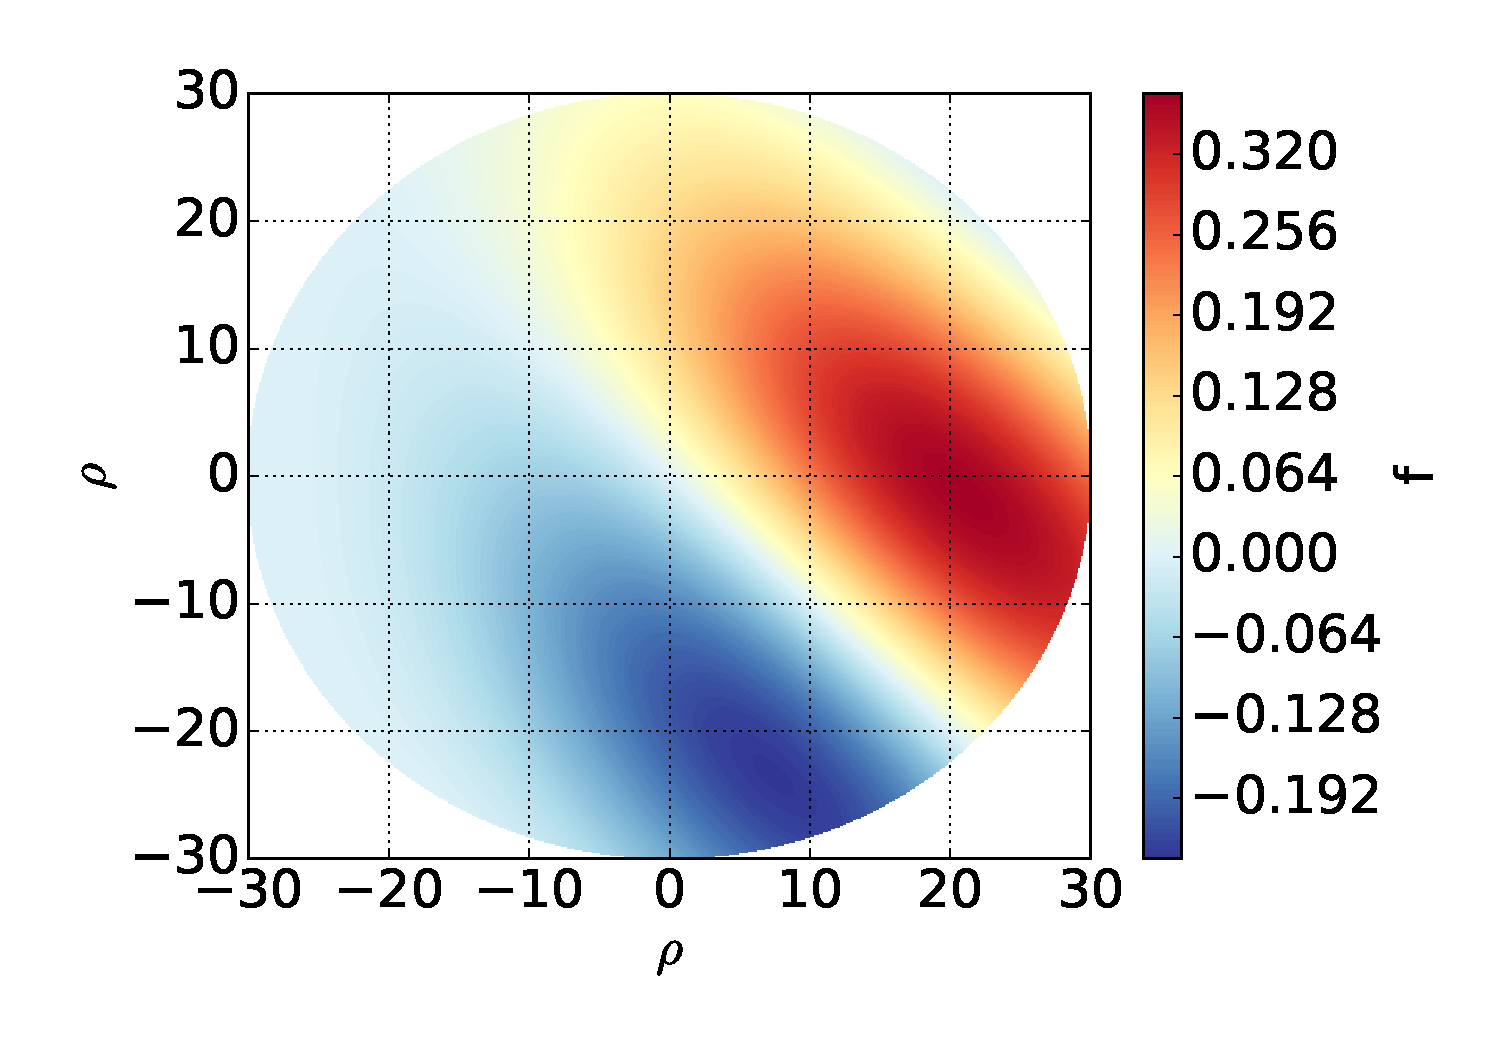
\includegraphics[width=1.0\textwidth]{fig/f}
        \caption{The function used in the MES}
    \end{subfigure}%
    ~
    \begin{subfigure}[t]{0.45\textwidth}
        \centering
        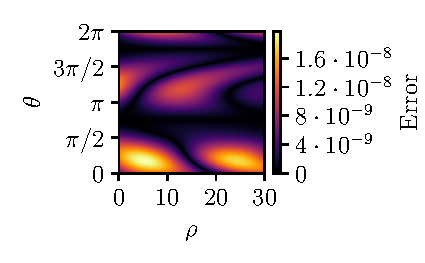
\includegraphics[width=1.0\textwidth]{fig/err}
        \caption{Typical plot of the errors}
    \end{subfigure}
    ~
    \begin{subfigure}[t]{0.45\textwidth}
        \centering
        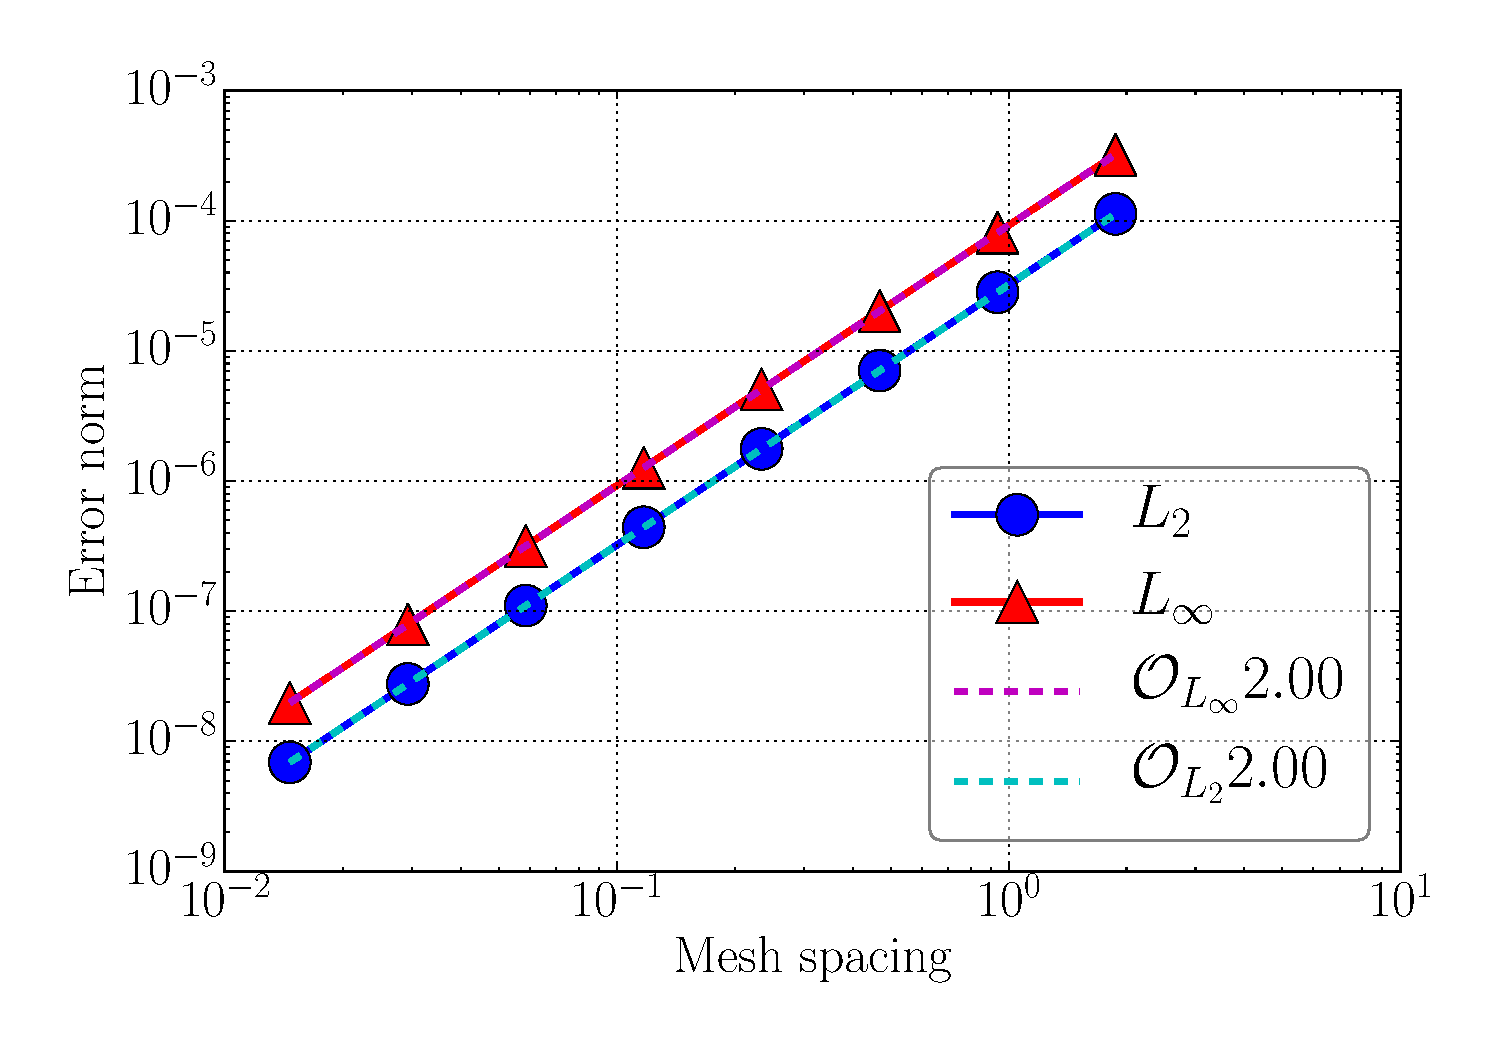
\includegraphics[width=1.0\textwidth]{fig/conv}
        \caption{Typical convergence plot}
    \end{subfigure}
    \caption{Typical function and errors for MES}
\end{figure}

\subsection{Single operators}
%
Although the single operators available from BOUT++ is verified in
\cite{Dudson2016}, the axis of a cylinder must be treated with care as there is
a singularity there ($J=0$ at $\rho=0$). To overcome this problem the
solution described in \cite{Naulin2008} has been used, and is illustrated in
figure \ref{fig:innerRho}.
%
\begin{figure}[htb]
    \centering
    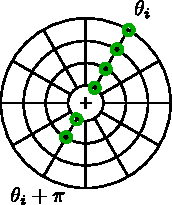
\includegraphics[width=0.3\textwidth]{fig/innerGhost}
    \caption{\textit{
        The green full circles represents the inner grid points at
        $\theta=\theta_i$. The green dashed circles at $\theta=\theta_i + \pi$
        are the ghost points (in the $\rho$-direction) belonging to the
        $\theta=\theta_i$ inner points. Equally the inner grid points at
        $\theta=\theta_i$ serves as ghost points (in the $\rho$-direction) for
        the inner points of $\theta=\theta_i + \pi$.
    }}
    \label{fig:innerRho}
\end{figure}
%
In this solution, the
the innermost ghost points%
\footnote{A grid point not belonging to the physical domain, but makes it
    possible to use a centered scheme when evaluating at the grid point closest
    to the physical boundary of the domain.}
in $\rho$ (closest to the singularity) with a
$\theta$ value lower
than (and excluding) $\pi$ will be set to the value of the innermost
internal point%
\footnote{A grid point which is not a ghost points, i.e. it belongs to the
    physical domain.}%
%
which lies
$\theta + \pi$ away. The next ghost point will be set to the value of the
second innermost internal point which lies $\theta + \pi$ away, and so on. In
this thesis, only one ghost point is used.

The convergence test for the single operators in $\rho$ direction can be found
in table \ref{tb:singleRho}.
%
\begin{table}[h!]
{\footnotesize \centerline{
\begin{tabular}{c|llllp{3cm}}
\hline\hline
Operation & $L_\inf$ order & $L_2$ order &
$L_\inf$ error ($2^{12}$ points) & $L_2$ error ($2^{12}$ points) & Comment\\
\hline
$\texttt{DDX}  (f)$ & $2.00$ & $2.00$ & $1.99\cdot10^{-8}$ & $6.90\cdot10^{-9}$& \\
$\texttt{D2DX2}(f)$ & $2.00$ & $2.00$ & $1.58\cdot10^{-9}$ & $5.07\cdot10^{-10}$& \\
$\texttt{D3DX3}(f)$ & $1.73$ & $2.00$ & $9.66\cdot10^{-10}$ & $1.57\cdot10^{-9}$&
$L_\inf$ order $=2$ until $2^{11}$ points
\\
$\texttt{D2DXDZ} (f)$ & $2.00$ & $2.00$ & $1.09\cdot10^{-8}$ & $2.97\cdot10^{-8}$& \\
$\texttt{D3DX2DZ}(f)$ & $2.00$ & $1.94$ & $2.33\cdot10^{-9}$ & $8.51\cdot10^{-10}$&
$L_\inf$ order $=2$ until $2^{11}$ points
\\
$\texttt{D3DZ2DX}(f)$ & $2.00$ & $2.00$ & $7.68\cdot10^{-8}$ & $2.88\cdot10^{-8}$& \\
$\texttt{DDX}   (Jf)$ & $2.00$ & $2.00$ & $5.22\cdot10^{-7}$ & $1.71\cdot10^{-7}$& \\
$\texttt{DDX}(\texttt{DDX}[f])$ & $-1.00$ & $-0.50$ & $1.67\cdot10^{0}$ & $2.60\cdot10^{-2}$&
Solution diverges. Errors dominating close to $\rho=0$.
\\
$\frac{\texttt{DDX}(f)}{J}$ & $1.00$ & $1.50$ & $3.16\cdot10^{-5}$ & $4.48\cdot10^{-7}$&
No order $2$nd order convergence. Errors dominating close to $\rho=0$.
\\
\hline\hline
\end{tabular}
}}
\caption[]{\textit{Convergence test of single operators in the $\rho$ direction}}
\protect\label{tb:singleRho}
\end{table}
%
For the cases where a convergence order of $2$ is found up until $2^{11}$
points, the schemes are considered convergent as the error is not dominating at
any particular point of the domain. In general, one can observe from the plots
of the error that they become a bit noisy in these cases, which could indicate
that machine precision in reached.

Note in the two last cases in table \ref{tb:singleRho} that the converge one
naively would have expected is generally not reached. In the case where we use
$\texttt{DDX}(\texttt{DDX}[f])$, the boundaries are reset after the first
operation. Notice that the resulting of stencil of these two operators is a
wide stencil. That is
%
\begin{align*}
D[D[f_i]] =& D\L[\frac{-f_{i-1} + f_{i+1}}{h_x}\R]
\\
=& \frac{-D[f_{i-1}] + D[f_{i+1}]}{h_x}
\\
=& \frac{-\frac{-f_{i-2} + f_{i}}{h_x} + \frac{-f_{i} + f_{i+2}}{h_x}}{h_x}
\\
=& \frac{f_{i-2} - 2f_{i} + f_{i+2}}{h_x^2}
\end{align*}
%
where $h_x$ denotes the grid spacing, and the subscript the grid index. Hence,
the observed divergence could be explained with poor information communication
across the singularity.

In the case of $\frac{\texttt{DDX}(f)}{J}$, the loss of expected convergence
rate can be explained by looking at the operator under investigation. As the
$\texttt{DDX}(f)$ operator used in this thesis is the standard $2$nd order
operator (obtained by subtracing the function Taylor expanded around $x_0$,
evaluated in $x+h$ from the function Taylor expanded around $x_0$,
evaluated in $x-h$ and divided by $2h$), one find that
%
\begin{align*}
    \deri{f}{x} - \texttt{DDX}(f) =
    \frac{h^2}{6}\deri{^2f}{x^2} + \mathcal{O}(h^3)
\end{align*}
%
In the first inner point $J=h_x$ as the boundaries lays half between the grid
points. Thus, in this point, we have that
%
\begin{align*}
    \frac{ \L.\deri{f}{x} \R|_{\text{first} \rho}}{J}
    - \frac{\L. \texttt{DDX}(f)\R|_{\text{first} \rho}}{J}=
    \frac{h}{6}\deri{^2f}{x^2} + \mathcal{O}(h^2)
\end{align*}
%
Thus for the first inner point, the scheme is not $2$nd order convergent.

Only one extra operator is implemented in the $\theta$-direction. This is shown
in table \ref{tb:singleZ}. Note that we use spectral methods in the $\theta$
direction, which is know to give minimal error. Machine precision is therefore
quickly reached, and performing MES after machine precision is nonsense due to
loss of percision when subtracting two amlost equal numbers. Indications that
machine precision is reached are low errors, and plots of the error appearing
noisy
%
\begin{table}[h!]
{\footnotesize \centerline{
\begin{tabular}{c|llllp{3cm}}
\hline\hline
Operation & $L_\inf$ order & $L_2$ order &
$L_\inf$ error ($2^{6}$ points) & $L_2$ error ($2^{6}$ points) & Comment\\
\hline
\texttt{D3DZ3}$(f)$ & $2.06$ & $2.10$ & $7.44\cdot10^{-11}$ & $7.33\cdot10^{-12}$&
Reaches machine precision at $2^6$.
\\
\hline\hline
\end{tabular}
}}
\caption[]{\textit{Convergence test single operators in the $\theta$ direction.}}
\protect\label{tb:singleZ}
\end{table}



\subsection{Divergence operators}
%           ▸ 1a-divPerp/
%           ▸ 1b-JTimesDivPerp/
%           ▸ 2a-divSource/
%           ▸ 2b-JTimesDivSource/
%           ▸ 3a-divExBAdv/
%           ▸ 3b-J4divExBAdv/

\subsection{The Naulin Solver}
% FIXME: Write about the function
functions here
mention BC
write implementation somewhere
\begin{table}[h!]
{\footnotesize \centerline{
        \begin{tabular}{lllll}
\hline\hline
$L_\inf$ order & $L_2$ order &
$L_\inf$ error ($2^{12}$ points) & $L_2$ error ($2^{12}$ points)\\
\hline
$2.00$ & $2.00$ & $3.19\cdot10^{-7}$ & $1.65\cdot10^{-7}$\\
\hline\hline
\end{tabular}
}}
\caption[]{\textit{Convergence test of the Naulin Solver in the $\rho$ direction}}
\protect\label{tb:naulinSolver}
\end{table}
%          ▸ Naulinsolver0Bndry/

\subsection{Boundary conditions}
%          ▸ 1-yExtrapolation/
%          ▸ 2-uEParSheath/
%          ▸ 3-cauchyBC/


\appendix

\chapter{The electrostatic approximation}
\label{app:elstat}
Rearranging \cref{fluideq:mom}, and multiplying it with $\frac{q_\a}{m_\a}$ yields
%
\begin{align*}
    q_{\a} \partial_t (n_{\a} \ve{u}_{\a})
    =&
    - q_{\a} \ve{u}_{\a} \partial_t n_{\a}
    - \frac{q_\a}{m_\a}\ve{u}_{\a}\cdot\nabla\ve{u}_{\a}
    - \frac{q_\a}{m_\a}\div \te{\pi}_{\a}
    - \frac{q_\a}{m_\a}\grad p_{\a}
    + \frac{q_\a^2}{m_\a} n_\a\L(\ve{E}  + \ve{u_\a}\times\ve{B}\R)
    \\ &
    + \frac{q_\a}{m_\a}\ve{R}_{\b\to \a}
    + \frac{q_\a}{m_\a}\ve{R}_{n\to \a}
    - q_\a S_{\a,n}\ve{u}_{\a}
\end{align*}
%
Adding the equation for electrons and ions using quasi-neutrality yields
%
\begin{align*}
    \partial_t \ve{J}
    =&
     \frac{\ve{J}}{n} \partial_t n
     \\&
    + \frac{e}{m_e}\ve{u}_{e}\cdot\nabla\ve{u}_{e}
    - \frac{e}{m_i}\ve{u}_{i}\cdot\nabla\ve{u}_{i}
     \\&
    + \frac{e}{m_e}\div \te{\pi}_{e}
    - \frac{e}{m_i}\div \te{\pi}_{i}
     \\&
    + \frac{e}{m_e}\grad p_{e}
    - \frac{e}{m_i}\grad p_{i}
     \\&
     + \frac{e^2}{m_e} n\L(-\grad{\phi}-\partial_t \ve{A}+ \ve{u_e}\times\ve{B}\R)
     + \frac{e^2}{m_i} n\L(-\grad{\phi}-\partial_t \ve{A}+ \ve{u_i}\times\ve{B}\R)
    \\ &
    - \frac{e}{m_e}\ve{R}_{i\to e}
    + \frac{e}{m_i}\ve{R}_{e\to i}
     \\&
    - \frac{e}{m_e}\ve{R}_{n\to e}
    + \frac{e}{m_i}\ve{R}_{n\to i}
     \\&
     + S \frac{\ve{J}}{n}
     \numberthis
     \label{eq:current_eq}
\end{align*}
%
where $\curl\ve{A}=\ve{B}$.
We then have that
%
\begin{align*}
    \curl\curl\ve{A}=&\curl\ve{B}
    \note{Low frequency}
    \\
    \grad^2\ve{A} - \grad(\div \ve{A})=&\mu_0\ve{J}
    \note{Coloumb gauge}
    % NOTE: See Griffiths
    \\
    \frac{\grad^2\ve{A}}{\mu_0}=&\ve{J}
    \\
    \ve{J} =& \frac{\div(\grad_\perp\ve{A}+\grad_\|\ve{A})}{\mu_0}
    \note{Assume $k_\perp \ll k_\|$}
    \\
    \ve{J} \simeq& \frac{\grad^2_\perp\ve{A}}{\mu_0}
    \numberthis
    \label{eq:coloumbGauge}
\end{align*}
%
Thus the LHS can be written
%
\begin{align*}
    \partial_t \ve{J} \simeq \partial_t \frac{\grad^2_\perp\ve{A}}{\mu_0}
\end{align*}
%
We can now use order of magnitude arguments to compare the size of the terms $\partial_t \frac{\grad^2_\perp\ve{A}}{\mu_0}$ and $\frac{e^2}{m_e}\partial_t \ve{A}$.
If the latter is larger than the former, it will mean that the time change of the magnetic field $\ve{B}$ will be a major contributor to the time change of the current $\ve{J}$, and electromagnetic effects be important%
%
\footnote{
    If the $\partial_t \ve{J}$ term was dominating (preferably by orders of magnitude), then there would be terms (or sum of terms) in \cref{eq:current_eq} which would be dominating the electromagnetic terms.
    Conversely, if the electromagnetic term was dominating, then the electromagnetic term would be dominating the sum of the other terms (not necessarily larger than each individual term, as terms may approximately cancel).
}.%
%
That is if
%
\begin{align*}
    \partial_t \frac{\grad^2_\perp\ve{A}}{\mu_0}
    < &
    \frac{ne^2}{m_e}\partial_t \ve{A}
    \\
    \rightarrow &
    \\
    \frac{1}{\omega_{ci}} \frac{k_\perp^2\ve{A}}{\mu_0}
    < &
    \frac{ne^2}{m_e}\frac{1}{\omega_{ci}} \ve{A}
    \\
    \frac{k_\perp^2}{\mu_0}
    < &
    \frac{ne^2}{m_e}
    \\
    k_\perp^2
    < &
    \frac{\mu_0ne^2}{m_e}
    \\
    k_\perp^2
    < &
    \frac{2m_i}{2m_i}\frac{B^2}{T_e}\frac{T_e}{B^2}\frac{\mu_0ne^2}{m_e}
    \\
    k_\perp^2
    < &
    \frac{m_i}{2m_e}\frac{e^2B^2}{m_iT_e}\frac{2\mu_0nT_e}{B^2}
    \\
    k_\perp^2
    < &
    \frac{m_i}{2m_e}\frac{1}{\rho_s^2}\b
\end{align*}
%
where the plasma beta ($\b$) is the kinetic pressure over the magnetic pressure.
As $ k_\perp^2\rho_s^2$ is typically in the order of unity for drift wave turbulence, we find that electromagnetic effects becomes important whenever
%
\begin{align*}
    1
    < &
    \frac{m_i}{2m_e}\b
    \\
    \frac{2m_e}{m_i}
    < &
    \b
\end{align*}
%
We observe that we get the identical condition if we choose to compare with $\frac{\ve{J}}{n}\partial_t n$ instead.
%FIXME; Consider to compare with other terms as well


\chapter{Clebsch coordinate system}
\label{app:Clebsch}
FIXME: Not Clebsch
In this thesis, we will use a Clebsch coordinate system which is defined in the
following way
%
\begin{align*}
    \ve{B}
    =&\ve{e}^3 \times \ve{e}^1\\
    J^{-1}\ve{e}_2=&\ve{e}^3 \times \ve{e}^1
\end{align*}
%
We have
%
\begin{align*}
    B\defined & \sqrt{\ve{B}\cdot\ve{B}}
    = \sqrt{J^{-1}\ve{e}_2\cdot J^{-1}\ve{e}_2}
    = \sqrt{J^{-2}g_{22}}
    = J^{-1}\sqrt{g_{22}}
\end{align*}
%
Which gives
%
\begin{align*}
    \ve{B}=&B\ve{b}\\
    \ve{b}=&\frac{\ve{B}}{B}
          =\frac{J^{-1}\ve{e}_2}{J^{-1}\sqrt{g_{22}}}
          =\frac{\ve{e}_2}{\sqrt{g_{22}}}
\end{align*}


\chapter{Cylindrical coordinate system}
\label{app:cylcoord}
The coordinates in a cylindrical geometry are written\\
%
\begin{minipage}{0.4\textwidth}
\begin{align*}
    x=&\rho \cos\theta\\
    y=&\rho \sin\theta\\
    z=& z
\end{align*}
\end{minipage}
\hfill
\begin{minipage}{0.4\textwidth}
\begin{align*}
    \rho=& \sqrt{x^2+y^2}\\
    \theta=&\atan\L(\frac{y}{x}\R)\\
    z=& z
\end{align*}
\end{minipage}

\section{In Clebsch formalism}
%
FIXME: Not Clebsch
The cylindrical coordinates can be expressed in Clebsch formalism introduced in appendix \ref{app:cylcoord} if we let
%
\begin{align*}
    1 &\to \rho\\
    2 &\to z\\
    3 &\to \theta
\end{align*}
%

\subsubsection{In BOUT++}
%
As a final note BOUT++ uses the indices $\{x,y,z\}$ rather than $\{1,2,3\}$.
Be aware that this can be a source of confusion as $y$ maps to $z$ as shown below
%
\begin{center}
    \begin{tabular}{ccccc}
        Generic &     & BOUT++ indices &     & Cylindrical coordinates\\
        $1$     &$\to$& $x$            &$\to$& $\rho$                 \\
        $2$     &$\to$& $y$            &$\to$& $z$                    \\
        $3$     &$\to$& $z$            &$\to$& $\theta$
    \end{tabular}
\end{center}
%

\section{The metrics}
\label{sec:metr}
%
We have that
%
\begin{align*}
    &\ve{e}_i = \partial_i&
    &\ve{e}^i = \d u_i&
\end{align*}
%
where $u_i$ is the set of the coordinate curves

To coordinate transform a covariant basis vector, we can consider an arbitrary line $f$ passing through the point under consideration written in the new set of coordinates.
We then use the chain rule to determine how the basis vector is written in the new set of coordinates.
We have
%
\begin{align*}
    \parti{f(\rho, \theta, z)}{x_i}
    =
    \parti{f}{\rho} \parti{\rho}{x_i}
    + \parti{f}{\theta} \parti{\theta}{x_i}
    + \parti{f}{z} \parti{z}{x_i}
\end{align*}
%
as the line $f$ is arbitrary, we have
%
\begin{align*}
    \ve{e}_i
    =
    \parti{}{x_i}
    =
    %
    \parti{\rho}{x_i} \parti{}{\rho}
    + \parti{\theta}{x_i} \parti{}{\theta}
    + \parti{z}{x_i} \parti{}{z}
    %
    =
    %
    \parti{\rho}{x_i} \ve{e}_{\rho}
    + \parti{\theta}{x_i} \ve{e}_{\theta}
    + \parti{z}{x_i} \ve{e}_{z}
    %
\end{align*}
%
where in our case $x_i \in \{x,y,z\}$.

To coordinate transform a contravariant basis vector, we can apply the chain rule directly to determine how the basis vector is written in the new set of coordinates.
We have
%
\begin{align*}
    \ve{e}^i
    =
    \d u^i(x,y,z)
    =
    %
    \parti{u_i}{x}\d x
    + \parti{u_i}{y}\d y
    + \parti{u_i}{z}\d z
    %
    =
    %
    \parti{u_i}{x}\ve{e}^x
    + \parti{u_i}{y}\ve{e}^y
    + \parti{u_i}{z}\ve{e}^z
    %
\end{align*}
%
At this point we note that there are no difference between co and contravariant basis vectors in a Cartesian coordinate system.

In the following, we are going to make use of the following relations
\\
%
\begin{minipage}{0.4\textwidth}
\begin{align*}
    \partial_x \rho
    =&
    \partial_x \sqrt{x^2+y^2}
    =
    \frac{x}{\rho}
    =
    \cos\theta\\
    %
    \partial_y \rho
    =&
    \partial_y \sqrt{x^2+y^2}
    =
    \frac{y}{\rho}
    =
    \sin\theta
    \\
    %
    \partial_z \rho
    =&
    \partial_z \sqrt{x^2+y^2}
    =
    0
    \\
    %
    %
    \partial_x \theta
    =&
    \partial_x \atan\L(\frac{y}{x}\R)
    =
    -\frac{y}{\rho^2}
    =
    -\frac{1}{\rho}\sin\theta
    \\
    %
    \partial_y \theta
    =&
    \partial_y \atan\L(\frac{y}{x}\R)
    =
    \frac{x}{\rho^2}
    =
    \frac{1}{\rho}\cos\theta
    \\
    %
    \partial_z \theta
    =&
    \partial_z \atan\L(\frac{y}{x}\R)
    =
    0
    \\
\end{align*}
\end{minipage}
%
\hfill
%
\begin{minipage}{0.4\textwidth}
\begin{align*}
    \partial_\rho x
    =&
    \partial_\rho \rho\cos\theta
    =
    \cos\theta\\
    %
    \partial_\rho y
    =&
    \partial_\rho \rho\sin\theta
    =
    \sin\theta
    \\
    %
    \partial_\rho z
    =&
    0
    \\
    %
    %
    \partial_\theta x
    =&
    \partial_\theta \rho\cos\theta
    =
    -\rho\sin\theta
    \\
    %
    \partial_\theta y
    =&
    \partial_\theta \rho\sin\theta
    =
    \rho\cos\theta
    \\
    %
    \partial_\theta z
    =&
    0
\end{align*}
\end{minipage}\\
%
This means that a basis vector written in a Cartesian basis can be written with a covariant basis vector using cylindrical coordinates as
%
\begin{align*}
    \ve{e}_x
    &=
    \parti{\rho}{x} \ve{e}_{\rho}
    + \parti{\theta}{x} \ve{e}_{\theta}
    + \parti{z}{x} \ve{e}_{z}
    %
    =
    \cos\theta \ve{e}_\rho
    - \frac{1}{\rho} \sin\theta \ve{e}_\theta
    \\
%
%
    \ve{e}_y
    &=
    \parti{\rho}{y} \ve{e}_{\rho}
    + \parti{\theta}{y} \ve{e}_{\theta}
    + \parti{z}{y} \ve{e}_{z}
    %
    =
    \sin\theta \ve{e}_\rho
    + \frac{1}{\rho} \cos\theta \ve{e}_\theta
    \\
%
%
    \ve{e}_z
    &=
    \parti{\rho}{z} \ve{e}_{\rho}
    + \parti{\theta}{z} \ve{e}_{\theta}
    + \parti{z}{z} \ve{e}_{z}
    %
    =
    \ve{e}_z
\end{align*}
%
For the back transformation we have
%
\begin{align*}
    \ve{e}_\rho
    &=
    \parti{x}{\rho} \ve{e}_{x}
    + \parti{y}{\rho} \ve{e}_{y}
    + \parti{z}{\rho} \ve{e}_{z}
    %
    =
    \cos\theta \ve{e}_x
    + \sin\theta \ve{e}_y
    \\
%
%
    \ve{e}_\theta
    &=
    \parti{x}{\theta} \ve{e}_{x}
    + \parti{y}{\theta} \ve{e}_{y}
    + \parti{z}{\theta} \ve{e}_{z}
    %
    =
    -\rho\sin\theta \ve{e}_x
    + \rho\cos\theta \ve{e}_y
    \\
%
%
    \ve{e}_z
    &=
    \parti{x}{z} \ve{e}_{x}
    + \parti{y}{z} \ve{e}_{y}
    + \parti{z}{z} \ve{e}_{z}
    %
    =
    \ve{e}_z
\end{align*}
%
Further, a basis vector written in a Cartesian basis can be written with a contravariant basis vector using cylindrical coordinates as
%
\begin{align*}
    \ve{e}^\rho
    &=
    \parti{\rho}{x} \ve{e}^{x}
    + \parti{\rho}{y} \ve{e}^{y}
    + \parti{\rho}{z} \ve{e}^{z}
    %
    =
    \cos\theta \ve{e}^x
    + \sin\theta \ve{e}^y
    \\
%
%
    \ve{e}^\theta
    &=
    \parti{\theta}{x} \ve{e}^{x}
    + \parti{\theta}{y} \ve{e}^{y}
    + \parti{\theta}{z} \ve{e}^{z}
    %
    =
    -\frac{1}{\rho}\sin\theta \ve{e}^x
    + \frac{1}{\rho} \cos\theta \ve{e}^y
    \\
%
%
    \ve{e}^z
    &=
    \parti{z}{x} \ve{e}^{x}
    + \parti{z}{y} \ve{e}^{y}
    + \parti{z}{z} \ve{e}^{z}
    %
    =
    \ve{e}^z
\end{align*}
%
The covariant metric tensor $g^{ij}=\ve{e}^i\cdot\ve{e}^j$ and the contravariant metric tensor $g_{ij}=\ve{e}_i\cdot\ve{e}_j$ can now be computed.
For the contravariant components, we get
%
\begin{align*}
    g^{\rho\rho}
    =&
    \L(
      \cos\theta\ve{e}^x
      + \sin\theta\ve{e}^y
    \R)
    \cdot
    \L(
      \cos\theta\ve{e}^x
      + \sin\theta\ve{e}^y
    \R)
    =
      \cos^2\theta
      + \sin^2\theta
    =
    1
    \\
    %
    g^{\rho\theta}
    =&
    g^{\theta\rho}
    =
    \L(
      \cos\theta\ve{e}^x
      + \sin\theta\ve{e}^y
    \R)
    \cdot
    \L(
      -\frac{1}{\rho}\cos\theta\ve{e}^x
      + \frac{1}{\rho}\sin\theta\ve{e}^y
    \R)
    =
      -\frac{1}{\rho}\cos\theta\sin\theta
      + \frac{1}{\rho}\sin\theta\cos\theta
    =
    0
    \\
    %
    g^{\rho z}
    =&
    g^{z \rho}
    =
    \L(
      \cos\theta\ve{e}^x
      + \sin\theta\ve{e}^y
    \R) \cdot \ve{e}^z = 0
    \\
    %
    %
    %
    g^{\theta\theta}
    =&
    \L(
      -\frac{1}{\rho}\cos\theta\ve{e}^x
      + \frac{1}{\rho}\sin\theta\ve{e}^y
    \R)
    \cdot
    \L(
      -\frac{1}{\rho}\cos\theta\ve{e}^x
      + \frac{1}{\rho}\sin\theta\ve{e}^y
    \R)
    =
      \frac{1}{\rho^2}\cos^2\theta
      + \frac{1}{\rho^2}\sin^2\theta
    =
    \frac{1}{\rho^2}
    \\
    %
    g^{z\theta}
    =&
    g^{\theta z}
    =
    \L(
      -\frac{1}{\rho}\cos\theta\ve{e}^x
      + \frac{1}{\rho}\sin\theta\ve{e}^y
    \R) \cdot \ve{e}^z = 0
    \\
    %
    %
    %
    g^{z z}
    =&
    \ve{e}^z \cdot \ve{e}^z =1
\end{align*}
%
And for the covariant components, we get
%
\begin{align*}
    g_{\rho\rho}
    =&
    \L(
      \cos\theta\ve{e}_x
      + \sin\theta\ve{e}_y
    \R)
    \cdot
    \L(
      \cos\theta\ve{e}_x
      + \sin\theta\ve{e}_y
    \R)
    =
      \cos^2\theta
      + \sin^2\theta
    =
    1
    \\
    %
    g_{\rho\theta}
    =&
    g_{\theta\rho}
    =
    \L(
      \cos\theta\ve{e}_x
      + \sin\theta\ve{e}_y
    \R)
    \cdot
    \L(
      -\rho\sin\theta\ve{e}_x
      + \rho\cos\theta\ve{e}_y
    \R)
    =
      -\rho\cos\theta\sin\theta
      + \rho\sin\theta\cos\theta
    =
    0
    \\
    %
    g_{\rho z}
    =&
    g_{z \rho}
    =
    \L(
      \cos\theta\ve{e}_x
      + \sin\theta\ve{e}_y
    \R) \cdot \ve{e}_z = 0
    \\
    %
    %
    %
    g_{\theta\theta}
    =&
    \L(
      -\rho\sin\theta\ve{e}_x
      + \rho\cos\theta\ve{e}_y
    \R)
    \cdot
    \L(
      -\rho\sin\theta\ve{e}_x
      + \rho\cos\theta\ve{e}_y
    \R)
    =
      \rho^2\cos^2\theta
      + \rho^2\sin^2\theta
    =
    \rho^2
    \\
    %
    g_{z\theta}
    =&
    g_{\theta z}
    =
    \L( -\rho\sin\theta\ve{e}_x
      + \rho\cos\theta\ve{e}_y \R) \cdot \ve{e}_z
    =
    0
    \\
    %
    g_{z z} =&
    \ve{e}_z \cdot \ve{e}_z =1
\end{align*}
%
The Jacobian
%
\begin{align*}
    J=\sqrt{\det(g_{ij})}=\rho
\end{align*}
%
Using this metric, we get that
%
\begin{align*}
    &B = \frac{1}{\rho}&
    & \ve{b}= \ve{e}_z
\end{align*}
%
Finally, we calculate the derivatives of the contravariant basis vectors.
From what is calculated above, we see that $\partial_z e^i=0$ and $\partial_i e^z=0$.
The other basis vectors gives
%
\begin{align*}
    \partial_\rho \ve{e}^\theta
    &=&
    \partial_\rho
    \L( - \frac{1}{\rho} \sin\theta \ve{e}^x
        + \frac{1}{\rho} \cos\theta \ve{e}^y \R)
    =
        \frac{\sin\theta}{\rho^2} \ve{e}^x
        - \frac{\cos\theta}{\rho^2} \ve{e}^y
    =
    - \frac{1}{\rho}
    \L( - \frac{1}{\rho} \sin\theta \ve{e}^x
        + \frac{1}{\rho} \cos\theta \ve{e}^y \R)
    &=&
    - \frac{1}{\rho} \ve{e}^\theta
    \\
    %
    \partial_\rho \ve{e}^\rho
    &=&
    \partial_\rho
    \L( \cos\theta \ve{e}^x
        + \sin\theta \ve{e}^y \R)
    &=&
    0
    \\
    %
    \partial_\theta \ve{e}^\theta
    &=&
    \partial_\theta
    \L( - \frac{1}{\rho} \sin\theta \ve{e}^x
        + \frac{1}{\rho} \cos\theta \ve{e}^y \R)
    =
    \L( - \frac{1}{\rho} \cos\theta \ve{e}^x
        - \frac{1}{\rho} \sin\theta \ve{e}^y \R)
    =
    - \frac{1}{\rho}
    \L( \cos\theta \ve{e}^x
        + \sin\theta \ve{e}^y \R)
    &=&
    - \frac{1}{\rho}
    \ve{e}^\rho
    \\
    %
    \partial_\theta \ve{e}^\rho
    &=&
    \partial_\theta
    \L( \cos\theta \ve{e}^x
        + \sin\theta \ve{e}^y \R)
    =
        - \sin\theta \ve{e}^x
        + \cos\theta \ve{e}^y
    =
    \rho
    \L( - \frac{1}{\rho} \sin\theta \ve{e}^x
        + \frac{1}{\rho} \cos\theta \ve{e}^y \R)
    &=&
    \rho
    \ve{e}^\theta
\end{align*}
%

\section{Summary}
\label{app:cylSummary}
%
Basis vector transformations\\
%
\begin{minipage}{0.3\textwidth}
\begin{align*}
    \ve{e}_x
    &=
    \cos\theta \ve{e}_\rho
    - \frac{1}{\rho} \sin\theta \ve{e}_\theta
    \\
%
%
    \ve{e}_y
    &=
    \sin\theta \ve{e}_\rho
    + \frac{1}{\rho} \cos\theta \ve{e}_\theta
    \\
%
%
    \ve{e}_z &= \ve{e}_z
\end{align*}
\end{minipage}
%
\hfill
%
\begin{minipage}{0.3\textwidth}
    \begin{align*}
        \ve{e}_\rho
        &=
        \cos\theta \ve{e}_x
        + \sin\theta \ve{e}_y
        \\
    %
    %
        \ve{e}_\theta
        &=
        -\rho\sin\theta \ve{e}_x
        + \rho\cos\theta \ve{e}_y
        \\
    %
    %
        \ve{e}_z &= \ve{e}_z
    \end{align*}
\end{minipage}
%
\hfill
%
\begin{minipage}{0.3\textwidth}
    \begin{align*}
        \ve{e}^\rho
        &=
        \cos\theta \ve{e}^x
        + \sin\theta \ve{e}^y
        \\
    %
    %
        \ve{e}^\theta
        &=
        -\frac{1}{\rho}\sin\theta \ve{e}^x
        + \frac{1}{\rho} \cos\theta \ve{e}^y
        \\
    %
    %
        \ve{e}^z &= \ve{e}^z
    \end{align*}
\end{minipage}
\\
%
Metric tensors
%
\begin{align*}
    &
    g^{\rho\theta} = g^{\theta\rho}
    = g^{\rho z} = g^{z \rho}
    = g^{z\theta} = g^{\theta z}
    = 0
    &
    &
    g_{\rho\theta} = g_{\theta\rho}
    = g_{\rho z} = g_{z \rho}
    = g_{z\theta} = g_{\theta z}
    = 0
    &
    \\
    &
    g^{\rho\rho} = g^{z z} = 1
    &
    &
    g_{\rho\rho} = g_{z z} = 1
    &
    \\
    %
    &
    g^{\theta\theta} = \frac{1}{\rho^2}
    &
    &
    g_{\theta\theta} = \rho^2
    &
\end{align*}
%
The Jacobian
%
\begin{align*}
    J=\rho
\end{align*}
%
The magnetic filed
%
\begin{align*}
    &B = \frac{1}{\rho}&
    & \ve{b}= \ve{e}_z
\end{align*}
%
The derivatives of the contravariant basis vectors.
\begin{align*}
    \partial_\rho \ve{e}^\rho =&
    \partial_\rho \ve{e}^z =
    \partial_\theta \ve{e}^z =
    \partial_z \ve{e}^\rho =
    \partial_z \ve{e}^\theta =
    \partial_z \ve{e}^z = 0
    \\
    %
    \partial_\rho \ve{e}^\theta =& - \frac{1}{\rho} \ve{e}^\theta
    \\
    %
    \partial_\theta \ve{e}^\theta =& - \frac{1}{\rho} \ve{e}^\rho
    \\
    %
    \partial_\theta \ve{e}^\rho =& \rho \ve{e}^\theta
\end{align*}


\chapter{The Poisson bracket operator}
\label{app:poisson}
We will here derive the bracket operators used for perpendicular advection.
Under electrostatic conditions, we have that $\ve{u}_{E, \text{with Clebsch B}} = -\frac{\nabla\phi\times\ve{b}_\text{Clebsch}}{B_\text{Clebsch}}$, which is similar to $\ve{u}=\ve{k}\times\nabla\psi$ found in incompressible fluid flow
%
\begin{align*}
    \ve{u}_{E, \text{with Clebsch B}} =& -\frac{\nabla\phi\times\ve{b}_\text{Clebsch}}{B_\text{Clebsch}}\\
         %
         =&-\frac{\nabla\phi\times\ve{e}_2}{
               \sqrt{g_{22}}J^{-1}\sqrt{g_{22}}}\\
             %
         =&-\frac{J}{g_{22}}\nabla\phi\times\ve{e}_2\\
         %
         =&\frac{J}{g_{22}}\ve{e}_2\times\nabla\phi\\
         %
         =&\frac{J}{g_{22}}\ve{e}_2\times
           \L(\ve{e}^1\partial_1 + \ve{e}^3\partial_3\R)\phi\\
         %
         =&\frac{J}{g_{22}}
           \L(g_{21}\ve{e}^1 + g_{22}\ve{e}^2 + g_{23}\ve{e}^3\R)
           \times
           \L(\ve{e}^1\partial_1 +
              \ve{e}^2\partial_2 +
                  \ve{e}^3\partial_3\R)\phi\\
             %
         =&\frac{J}{g_{22}}
           \L(
             g_{21}\ve{e}^1\times\ve{e}^1\partial_1
           + g_{22}\ve{e}^2\times\ve{e}^1\partial_1
           + g_{23}\ve{e}^3\times\ve{e}^1\partial_1
           \R.
           \\
           &\quad\;
           + g_{21}\ve{e}^1\times\ve{e}^2\partial_2
           + g_{22}\ve{e}^2\times\ve{e}^2\partial_2
           + g_{23}\ve{e}^3\times\ve{e}^2\partial_2
           \\
           &\quad\;
           \L.
           + g_{21}\ve{e}^1\times\ve{e}^3\partial_3
           + g_{22}\ve{e}^2\times\ve{e}^3\partial_3
           + g_{23}\ve{e}^3\times\ve{e}^3\partial_3
           \R)
           \phi\\
         %
         =&\frac{J}{g_{22}}
           \L(
           - g_{22}\ve{e}^2\times\ve{e}^1\partial_1
           + g_{23}\ve{e}^3\times\ve{e}^1\partial_1
           \R.
           \\
           &\quad
           + g_{21}\ve{e}^1\times\ve{e}^2\partial_2
           - g_{23}\ve{e}^3\times\ve{e}^2\partial_2
           \\
           &\quad
           \L.
           - g_{21}\ve{e}^1\times\ve{e}^3\partial_3
           + g_{22}\ve{e}^2\times\ve{e}^3\partial_3
           \R)
           \phi\\
         %
         =&\frac{1}{g_{22}}
           \L(
           - g_{22}\ve{e}_3\partial_1
           + g_{23}\ve{e}_2\partial_1
           + g_{21}\ve{e}_3\partial_2
           - g_{23}\ve{e}_1\partial_2
           - g_{21}\ve{e}_2\partial_3
           + g_{22}\ve{e}_1\partial_3
           \R)
           \phi.
           \numberthis
           \label{poi:ExB}
\end{align*}
%
We note that \cref{poi:ExB} is derived for a system where we are using $B_\text{Clebsch}$.
Translating this into a cylindrical coordinate system using $B_\text{Cylindrical}$ gives
%
\begin{align*}
    \ve{u}_{E, \text{with constant B}} =&
    -\frac{\nabla\phi\times\ve{b}_\text{Clebsch}}{B_\text{Cylinder}}
    \\
    %
= &
    -\frac{B_\text{Clebsch}}{B_\text{Clebsch}}\frac{\nabla\phi\times\ve{b}_\text{Clebsch}}{B_\text{Cylinder}}
    \\
%
= &
    -\frac{B_\text{Clebsch}}{B_\text{Cylinder}}\frac{\nabla\phi\times\ve{b}_\text{Clebsch}}{B_\text{Clebsch}}
    \\
%
= &
    \frac{\sqrt{g_{zz}}}{JB_\text{Cylinder}}
    \ve{u}_{E, \text{with Clebsch B}}
    \\
%
= &
    \frac{1}{JB_\text{Cylinder}}
         \frac{1}{g_{zz}}
           \L(
           - g_{z z}\ve{e}_\theta\partial_\rho
           + g_{z\theta}\ve{e}_ z\partial_\rho
           + g_{z\rho}\ve{e}_\theta\partial_z
           - g_{z\theta}\ve{e}_\rho\partial_z
           - g_{z\rho}\ve{e}_ z\partial_\theta
           + g_{z z}\ve{e}_\rho\partial_\theta
           \R)
           \phi
    \\
%
= &
    \frac{1}{JB_\text{Cylinder}}
           \L(
           - \ve{e}_\theta\partial_\rho
           + \ve{e}_\rho\partial_\theta
           \R)
           \phi.
    \numberthis
    \label{poi:cylExB}
\end{align*}
%
Continuing from \cref{poi:ExB}, we see that in general coordinates the electrostatic $\ve{E}\times \ve{B}$ advection operator becomes
%
\begin{align*}
    \ve{u}_{E, \text{with Clebsch B}}\cdot\nabla
    =& -\frac{\nabla\phi\times\ve{b}_\text{Clebsch}}{B_\text{Clebsch}}\cdot\nabla\\
    %
    %
    =&\frac{1}{g_{22}}
           \L(
           - g_{22}\ve{e}_3\partial_1
           + g_{23}\ve{e}_2\partial_1
           + g_{21}\ve{e}_3\partial_2
           - g_{23}\ve{e}_1\partial_2
           - g_{21}\ve{e}_2\partial_3
           + g_{22}\ve{e}_1\partial_3
           \R)
           \phi
           \\
           &
       \cdot\L(\ve{e}^1\partial_1 + \ve{e}^2\partial_2 + \ve{e}^3\partial_3\R)\\
    %
    %
    =& \frac{1}{g_{22}}
           \L(
           - g_{22}\partial_1\phi\partial_3
           + g_{23}\partial_1\phi\partial_2
           + g_{21}\partial_2\phi\partial_3
           - g_{23}\partial_2\phi\partial_1
           - g_{21}\partial_3\phi\partial_2
           + g_{22}\partial_3\phi\partial_1
           \R)\\
    %
    %
    =& \frac{1}{g_{22}}
           \L(
             \L[
               g_{22}\partial_3\phi
             - g_{23}\partial_2\phi
             \R]\partial_1
           +
             \L[
               g_{23}\partial_1\phi
             - g_{21}\partial_3\phi
             \R]\partial_2
           +
             \L[
               g_{21}\partial_2\phi
             - g_{22}\partial_1\phi
             \R]\partial_3
           \R)\\
    %
    %
    =& \frac{1}{g_{22}}
               \L(
                 g_{21}\{\phi, \cdot\}_{2,3}
                 +
                 g_{22}\{\phi, \cdot\}_{3,1}
                 +
                 g_{23}\{\phi, \cdot\}_{1,2}
              \R),
\end{align*}
%
where we have used the definition of the Poisson bracket
%
\begin{align*}
    \{f, g\}_{i,j} = \L(\partial_i f\R) \partial_j g - \L(\partial_j f\R) \partial_i g.
\end{align*}
%
In an orthogonal system, all the off diagonal elements are zero, so
%
\begin{align}
    \ve{u}_{E, \text{with Clebsch B}}\cdot\nabla
    = \frac{1}{g_{22}} \L( g_{22}\{\phi, \cdot\}_{3,1} \R)
    = \{\phi, \cdot\}_{3,1}
    = \partial_3\phi\partial_1 - \partial_1\phi\partial_3
    = \partial_\theta\phi\partial_\rho - \partial_\rho\phi\partial_\theta.
    \label{poi:defClebsh}
\end{align}
%
As \cref{poi:defClebsh} is derived with $B_\text{Clebsch}$, we get that
%
\begin{align*}
    \ve{u}_{E, \text{with const B}}\cdot\nabla
    =& \frac{B_{\text{Clebsch}}}{B_{\text{Cylindrical}}}\ve{u}_{E, \text{with Clebsch B}}\cdot\nabla\\
    =& \frac{\sqrt{g_{zz}}}{JB_{\text{Cylindrical}}}
    (\partial_\theta\phi\partial_\rho - \partial_\rho\phi\partial_\theta)\\
    =& \frac{1}{JB}
    (\partial_\theta\phi\partial_\rho - \partial_\rho\phi\partial_\theta).
    \numberthis
    \label{poi:def}
\end{align*}


\markboth{Bibliography}{}
\bibliographystyle{bib/prsty}
\bibliography{bib/library,bib/nonArticles}
\addcontentsline{toc}{chapter}{Bibliography}

\end{document}
